\documentclass{article}
\def\submissionmode{1}
\def\anonsubmission{1}
% NeurIPS 2026 style. Build variants:
%   preprint (named, default):  \usepackage[preprint]{neurips_2026}
%   anonymous submission:       \usepackage{neurips_2026}
%   camera-ready:               \usepackage[final]{neurips_2026}
\ifdefined\anonsubmission
  \usepackage{neurips_2026}
\else
  \usepackage[preprint]{neurips_2026}
\fi
\usepackage[utf8]{inputenc}
\usepackage[T1]{fontenc}
\usepackage{hyperref}
\usepackage{url}
\usepackage{booktabs,tabularx,makecell,multirow}
\usepackage{amsmath,amssymb,amsfonts}
\usepackage{nicefrac}
\usepackage{microtype}
\usepackage{xcolor}
\usepackage{graphicx}
\usepackage{enumitem}
\usepackage{caption}
\usepackage{placeins}
\captionsetup{font=small,labelfont=bf}
\setlength{\tabcolsep}{4pt}

% Shared layout switches for the preprint (main.tex) and the anonymised submission (submission.tex).
\providecommand{\submissionmode}{0}
\newif\ifsubmission
\ifnum\submissionmode=1 \submissiontrue \else \submissionfalse \fi
% full-version-only material; the submission moves it to the appendix
\newcommand{\fullonly}[1]{\ifsubmission\else\input{#1}\fi}
\newcommand{\movable}[1]{\ifsubmission\else\input{#1}\fi}
\newcommand{\repourl}{\ifsubmission an anonymised repository (link withheld for review)\else\url{https://github.com/arghya05/jev-boundary-study}\fi}
\newcommand{\commitref}[1]{\ifsubmission\texttt{[hash withheld]}\else\texttt{#1}\fi}

% generated by jevstudy.paper_assets -- do not edit
\newcommand{\AbsDeltaAnliAstra}{10.7}
\newcommand{\AbsDeltaAnliFable}{13.1}
\newcommand{\AbsDeltaFolioAstra}{17.2}
\newcommand{\AbsDeltaFolioFable}{20.6}
\newcommand{\AbsDeltaHAnliAstra}{0.3}
\newcommand{\AbsDeltaHAnliFable}{2.8}
\newcommand{\AbsDeltaHCtlAstra}{3.1}
\newcommand{\AbsDeltaHCtlFable}{3.1}
\newcommand{\AbsDeltaHFolioAstra}{2.5}
\newcommand{\AbsDeltaHFolioFable}{5.9}
\newcommand{\AbsDeltaHHaluAstra}{2.9}
\newcommand{\AbsDeltaHHaluFable}{5.6}
\newcommand{\AbsDeltaHJbgptAstra}{6.4}
\newcommand{\AbsDeltaHJbgptFable}{6.1}
\newcommand{\AbsDeltaHRbAstra}{0.6}
\newcommand{\AbsDeltaHRbFable}{4.2}
\newcommand{\AbsDeltaHRbFableAnswered}{0.8}
\newcommand{\AbsDeltaHaluAstra}{7.9}
\newcommand{\AbsDeltaHaluFable}{10.6}
\newcommand{\AbsDeltaJbgptAstra}{26.3}
\newcommand{\AbsDeltaJbgptFable}{26.0}
\newcommand{\AbsDeltaRbAstra}{5.4}
\newcommand{\AbsDeltaRbFable}{1.8}
\newcommand{\AccAnliAstra}{74.9}
\newcommand{\AccAnliFable}{77.3}
\newcommand{\AccAnliHarn}{74.6}
\newcommand{\AccAnliSone}{64.2}
\newcommand{\AccCtlAstra}{100.0}
\newcommand{\AccCtlFable}{100.0}
\newcommand{\AccCtlHarn}{96.9}
\newcommand{\AccCtlSone}{55.9}
\newcommand{\AccCtlStwo}{100.0}
\newcommand{\AccFolioAstra}{86.8}
\newcommand{\AccFolioFable}{90.2}
\newcommand{\AccFolioHarn}{84.3}
\newcommand{\AccFolioSone}{69.6}
\newcommand{\AccFolioStwo}{85.8}
\newcommand{\AccHRbFableAnsweredF}{94.9}
\newcommand{\AccHRbFableAnsweredH}{94.1}
\newcommand{\AccHaluAstra}{90.6}
\newcommand{\AccHaluFable}{93.3}
\newcommand{\AccHaluHarn}{87.7}
\newcommand{\AccHaluSone}{82.7}
\newcommand{\AccJbgptAstra}{94.5}
\newcommand{\AccJbgptFable}{94.2}
\newcommand{\AccJbgptHarn}{88.2}
\newcommand{\AccJbgptSone}{68.2}
\newcommand{\AccRbAstra}{93.8}
\newcommand{\AccRbFable}{90.2}
\newcommand{\AccRbHarn}{94.4}
\newcommand{\AccRbSone}{87.0}
\newcommand{\ApiTotal}{65.04}
\newcommand{\BridgeDFive}{40.6}
\newcommand{\BridgeDFour}{42.3}
\newcommand{\BridgeDOne}{72.7}
\newcommand{\BridgeDThree}{56.8}
\newcommand{\BridgeDTwo}{57.3}
\newcommand{\BridgeDZero}{94.0}
\newcommand{\ChgAstraCtx}{-13.2}
\newcommand{\ChgAstraDfive}{-5.2}
\newcommand{\ChgAstraDthree}{-11.5}
\newcommand{\ChgFableCtx}{-13.2}
\newcommand{\ChgFableDfive}{-5.2}
\newcommand{\ChgFableDthree}{-11.5}
\newcommand{\ChgStwoDfive}{-5.2}
\newcommand{\ChgStwoDthree}{-11.5}
\newcommand{\ConclHAnliAstra}{inconclusive}
\newcommand{\ConclHAnliFable}{inconclusive}
\newcommand{\ConclHCtlAstra}{inconclusive}
\newcommand{\ConclHCtlFable}{inconclusive}
\newcommand{\ConclHFolioAstra}{inconclusive}
\newcommand{\ConclHFolioFable}{inconclusive}
\newcommand{\ConclHHaluAstra}{inconclusive}
\newcommand{\ConclHHaluFable}{frontier materially more accurate}
\newcommand{\ConclHJbgptAstra}{inconclusive}
\newcommand{\ConclHJbgptFable}{inconclusive}
\newcommand{\ConclHRbAstra}{inconclusive}
\newcommand{\ConclHRbFable}{JEV-H more accurate}
\newcommand{\CostAnliAstra}{7.00}
\newcommand{\CostAnliFable}{7.52}
\newcommand{\CostAnliHarn}{0.623}
\newcommand{\CostAnliSone}{0.045}
\newcommand{\CostCtlAstra}{5.65}
\newcommand{\CostCtlFable}{7.87}
\newcommand{\CostCtlHarn}{0.572}
\newcommand{\CostCtlSone}{0.037}
\newcommand{\CostCtlStwo}{0.609}
\newcommand{\CostFolioAstra}{8.97}
\newcommand{\CostFolioFable}{11.68}
\newcommand{\CostFolioHarn}{0.483}
\newcommand{\CostFolioSone}{0.041}
\newcommand{\CostFolioStwo}{0.609}
\newcommand{\CostHaluAstra}{2.45}
\newcommand{\CostHaluFable}{3.64}
\newcommand{\CostHaluHarn}{0.424}
\newcommand{\CostHaluSone}{0.096}
\newcommand{\CostJbgptAstra}{22.01}
\newcommand{\CostJbgptFable}{42.28}
\newcommand{\CostJbgptHarn}{1.19}
\newcommand{\CostJbgptSone}{0.153}
\newcommand{\CostRbAstra}{4.01}
\newcommand{\CostRbFable}{5.78}
\newcommand{\CostRbHarn}{0.654}
\newcommand{\CostRbSone}{0.170}
\newcommand{\CtlAstraAnswerChanged}{100}
\newcommand{\CtlAstraBaseAcc}{100}
\newcommand{\CtlAstraBothCorrect}{100}
\newcommand{\CtlAstraChangeAcc}{100}
\newcommand{\CtlAstraInvariant}{100}
\newcommand{\CtlAstraPreserveAcc}{100}
\newcommand{\CtlFableAnswerChanged}{100}
\newcommand{\CtlFableBaseAcc}{100}
\newcommand{\CtlFableBothCorrect}{100}
\newcommand{\CtlFableChangeAcc}{100}
\newcommand{\CtlFableInvariant}{100}
\newcommand{\CtlFablePreserveAcc}{100}
\newcommand{\CtlHarnAnswerChanged}{98}
\newcommand{\CtlHarnBaseAcc}{98}
\newcommand{\CtlHarnBothCorrect}{96}
\newcommand{\CtlHarnChangeAcc}{98}
\newcommand{\CtlHarnInvariant}{96}
\newcommand{\CtlHarnPreserveAcc}{98}
\newcommand{\CtlSoneAnswerChanged}{48}
\newcommand{\CtlSoneBaseAcc}{40}
\newcommand{\CtlSoneBothCorrect}{23}
\newcommand{\CtlSoneChangeAcc}{58}
\newcommand{\CtlSoneInvariant}{58}
\newcommand{\CtlSonePreserveAcc}{31}
\newcommand{\CtlStwoAnswerChanged}{100}
\newcommand{\CtlStwoBaseAcc}{100}
\newcommand{\CtlStwoBothCorrect}{100}
\newcommand{\CtlStwoChangeAcc}{100}
\newcommand{\CtlStwoInvariant}{100}
\newcommand{\CtlStwoPreserveAcc}{100}
\newcommand{\DeepAstraDFive}{100.0}
\newcommand{\DeepAstraDNine}{100.0}
\newcommand{\DeepAstraDOne}{100.0}
\newcommand{\DeepFableDFive}{100.0}
\newcommand{\DeepFableDNine}{100.0}
\newcommand{\DeepFableDOne}{100.0}
\newcommand{\DeepHarnDFive}{100.0}
\newcommand{\DeepHarnDNine}{100.0}
\newcommand{\DeepHarnDOne}{100.0}
\newcommand{\DeepSoneDFive}{62.5}
\newcommand{\DeepSoneDNine}{41.7}
\newcommand{\DeepSoneDOne}{62.5}
\newcommand{\DeepStwoDFive}{100.0}
\newcommand{\DeepStwoDNine}{95.8}
\newcommand{\DeepStwoDOne}{100.0}
\newcommand{\DeltaAnliAstra}{-10.7}
\newcommand{\DeltaAnliFable}{-13.1}
\newcommand{\DeltaFolioAstra}{-17.2}
\newcommand{\DeltaFolioFable}{-20.6}
\newcommand{\DeltaHAnliAstra}{-0.3}
\newcommand{\DeltaHAnliFable}{-2.8}
\newcommand{\DeltaHCtlAstra}{-3.1}
\newcommand{\DeltaHCtlFable}{-3.1}
\newcommand{\DeltaHFolioAstra}{-2.5}
\newcommand{\DeltaHFolioFable}{-5.9}
\newcommand{\DeltaHHaluAstra}{-2.9}
\newcommand{\DeltaHHaluFable}{-5.6}
\newcommand{\DeltaHJbgptAstra}{-6.4}
\newcommand{\DeltaHJbgptFable}{-6.1}
\newcommand{\DeltaHRbAstra}{0.6}
\newcommand{\DeltaHRbFable}{4.2}
\newcommand{\DeltaHRbFableAnswered}{-0.8}
\newcommand{\DeltaHaluAstra}{-7.9}
\newcommand{\DeltaHaluFable}{-10.6}
\newcommand{\DeltaJbgptAstra}{-26.3}
\newcommand{\DeltaJbgptFable}{-26.0}
\newcommand{\DeltaRbAstra}{-5.4}
\newcommand{\DeltaRbFable}{-1.8}
\newcommand{\DidAstraCtx}{-13.2}
\newcommand{\DidAstraDfive}{-5.2}
\newcommand{\DidAstraDthree}{-11.5}
\newcommand{\DidFableCtx}{-13.2}
\newcommand{\DidFableDfive}{-5.2}
\newcommand{\DidFableDthree}{-11.5}
\newcommand{\DidHiAstraCtx}{0.7}
\newcommand{\DidHiAstraDfive}{13.5}
\newcommand{\DidHiAstraDthree}{6.2}
\newcommand{\DidHiFableCtx}{0.7}
\newcommand{\DidHiFableDfive}{13.5}
\newcommand{\DidHiFableDthree}{6.2}
\newcommand{\DidHiStwoDfive}{8.3}
\newcommand{\DidHiStwoDthree}{1.0}
\newcommand{\DidLoAstraCtx}{-27.1}
\newcommand{\DidLoAstraDfive}{-24.0}
\newcommand{\DidLoAstraDthree}{-28.1}
\newcommand{\DidLoFableCtx}{-27.1}
\newcommand{\DidLoFableDfive}{-24.0}
\newcommand{\DidLoFableDthree}{-28.1}
\newcommand{\DidLoStwoDfive}{-18.8}
\newcommand{\DidLoStwoDthree}{-24.0}
\newcommand{\DidStwoDfive}{-5.2}
\newcommand{\DidStwoDthree}{-11.5}
\newcommand{\EscAnli}{80.8}
\newcommand{\EscCtl}{81.2}
\newcommand{\EscDeep}{88.9}
\newcommand{\EscFolio}{64.7}
\newcommand{\EscHalueval}{37.6}
\newcommand{\EscJudgebench}{90.5}
\newcommand{\EscRewardbench}{51.2}
\newcommand{\FlipCtlSone}{3.5}
\newcommand{\FlipFolioSone}{5.9}
\newcommand{\HaluLenAuroc}{0.976}
\newcommand{\HiAnliAstra}{-7.0}
\newcommand{\HiAnliFable}{-9.4}
\newcommand{\HiFolioAstra}{-7.2}
\newcommand{\HiFolioFable}{-12.1}
\newcommand{\HiHAnliAstra}{3.1}
\newcommand{\HiHAnliFable}{0.6}
\newcommand{\HiHCtlAstra}{-0.7}
\newcommand{\HiHCtlFable}{-0.7}
\newcommand{\HiHFolioAstra}{5.1}
\newcommand{\HiHFolioFable}{0.0}
\newcommand{\HiHHaluAstra}{-0.7}
\newcommand{\HiHHaluFable}{-3.3}
\newcommand{\HiHJbgptAstra}{-1.5}
\newcommand{\HiHJbgptFable}{-1.9}
\newcommand{\HiHRbAstra}{3.6}
\newcommand{\HiHRbFable}{8.2}
\newcommand{\HiHRbFableAnswered}{2.1}
\newcommand{\HiHaluAstra}{-5.5}
\newcommand{\HiHaluFable}{-8.1}
\newcommand{\HiJbgptAstra}{-17.2}
\newcommand{\HiJbgptFable}{-16.5}
\newcommand{\HiRbAstra}{-1.6}
\newcommand{\HiRbFable}{2.6}
\newcommand{\LatAstra}{2.68}
\newcommand{\LatFable}{1.93}
\newcommand{\LatNinetyfiveAstra}{8.66}
\newcommand{\LatNinetyfiveFable}{5.54}
\newcommand{\LatNinetyfiveSone}{0.10}
\newcommand{\LatSone}{0.08}
\newcommand{\LoAnliAstra}{-14.1}
\newcommand{\LoAnliFable}{-16.7}
\newcommand{\LoFolioAstra}{-26.6}
\newcommand{\LoFolioFable}{-29.0}
\newcommand{\LoHAnliAstra}{-3.9}
\newcommand{\LoHAnliFable}{-6.1}
\newcommand{\LoHCtlAstra}{-6.2}
\newcommand{\LoHCtlFable}{-6.2}
\newcommand{\LoHFolioAstra}{-9.6}
\newcommand{\LoHFolioFable}{-12.9}
\newcommand{\LoHHaluAstra}{-5.3}
\newcommand{\LoHHaluFable}{-8.2}
\newcommand{\LoHJbgptAstra}{-19.1}
\newcommand{\LoHJbgptFable}{-16.6}
\newcommand{\LoHRbAstra}{-2.4}
\newcommand{\LoHRbFable}{0.4}
\newcommand{\LoHRbFableAnswered}{-4.0}
\newcommand{\LoHaluAstra}{-10.4}
\newcommand{\LoHaluFable}{-13.3}
\newcommand{\LoJbgptAstra}{-32.8}
\newcommand{\LoJbgptFable}{-32.2}
\newcommand{\LoRbAstra}{-9.4}
\newcommand{\LoRbFable}{-6.4}
\newcommand{\NAnliAstra}{1200}
\newcommand{\NAnliFable}{1200}
\newcommand{\NAnliHarn}{1200}
\newcommand{\NAnliSone}{1200}
\newcommand{\NCtlAstra}{288}
\newcommand{\NCtlFable}{288}
\newcommand{\NCtlHarn}{288}
\newcommand{\NCtlSone}{288}
\newcommand{\NCtlStwo}{288}
\newcommand{\NFolioAstra}{204}
\newcommand{\NFolioFable}{204}
\newcommand{\NFolioHarn}{204}
\newcommand{\NFolioSone}{204}
\newcommand{\NFolioStwo}{204}
\newcommand{\NHaluAstra}{1000}
\newcommand{\NHaluFable}{1000}
\newcommand{\NHaluHarn}{1000}
\newcommand{\NHaluSone}{1000}
\newcommand{\NJbgptAstra}{346}
\newcommand{\NJbgptFable}{346}
\newcommand{\NJbgptHarn}{346}
\newcommand{\NJbgptSone}{346}
\newcommand{\NRbAstra}{500}
\newcommand{\NRbFable}{500}
\newcommand{\NRbHarn}{500}
\newcommand{\NRbSone}{2984}
\newcommand{\RbAstraChat}{86.7}
\newcommand{\RbAstraChatHard}{84.5}
\newcommand{\RbAstraReasoning}{100.0}
\newcommand{\RbAstraSafety}{91.0}
\newcommand{\RbFableChat}{96.7}
\newcommand{\RbFableChatHard}{87.3}
\newcommand{\RbFableReasoning}{100.0}
\newcommand{\RbFableSafety}{71.4}
\newcommand{\RbHarnChat}{93.3}
\newcommand{\RbHarnChatHard}{81.7}
\newcommand{\RbHarnReasoning}{98.7}
\newcommand{\RbHarnSafety}{94.0}
\newcommand{\RbSoneChat}{96.4}
\newcommand{\RbSoneChatHard}{67.5}
\newcommand{\RbSoneReasoning}{89.3}
\newcommand{\RbSoneSafety}{90.1}
\newcommand{\RbStwoChat}{81.8}
\newcommand{\RbStwoChatHard}{83.7}
\newcommand{\RbStwoReasoning}{98.6}
\newcommand{\RbStwoSafety}{87.2}
\newcommand{\RouteAstraAfrAcc}{90.1}
\newcommand{\RouteAstraAfrCost}{1.00}
\newcommand{\RouteAstraAfrWithin}{6/6}
\newcommand{\RouteAstraAjevAcc}{71.5}
\newcommand{\RouteAstraAjevCost}{0.01}
\newcommand{\RouteAstraAjevWithin}{0/6}
\newcommand{\RouteAstraFamAcc}{90.1}
\newcommand{\RouteAstraFamCost}{1.00}
\newcommand{\RouteAstraFamWithin}{6/6}
\newcommand{\RouteAstraGateAcc}{87.6}
\newcommand{\RouteAstraGateCost}{0.67}
\newcommand{\RouteAstraGateWithin}{4/6}
\newcommand{\RouteAstraLenAcc}{90.1}
\newcommand{\RouteAstraLenCost}{1.00}
\newcommand{\RouteAstraLenWithin}{6/6}
\newcommand{\RouteAstraOracleAcc}{93.4}
\newcommand{\RouteAstraOracleCost}{0.25}
\newcommand{\RouteAstraOracleWithin}{6/6}
\newcommand{\RouteAstraRuleAcc}{87.7}
\newcommand{\RouteAstraRuleCost}{0.84}
\newcommand{\RouteAstraRuleWithin}{4/6}
\newcommand{\RouteAstraRuleconfAcc}{89.3}
\newcommand{\RouteAstraRuleconfCost}{0.88}
\newcommand{\RouteAstraRuleconfWithin}{4/6}
\newcommand{\RouteFableAfrAcc}{90.9}
\newcommand{\RouteFableAfrCost}{1.00}
\newcommand{\RouteFableAfrWithin}{6/6}
\newcommand{\RouteFableAjevAcc}{71.5}
\newcommand{\RouteFableAjevCost}{0.01}
\newcommand{\RouteFableAjevWithin}{1/6}
\newcommand{\RouteFableFamAcc}{90.9}
\newcommand{\RouteFableFamCost}{1.00}
\newcommand{\RouteFableFamWithin}{6/6}
\newcommand{\RouteFableGateAcc}{88.5}
\newcommand{\RouteFableGateCost}{0.66}
\newcommand{\RouteFableGateWithin}{1/6}
\newcommand{\RouteFableLenAcc}{90.9}
\newcommand{\RouteFableLenCost}{1.00}
\newcommand{\RouteFableLenWithin}{6/6}
\newcommand{\RouteFableOracleAcc}{94.3}
\newcommand{\RouteFableOracleCost}{0.27}
\newcommand{\RouteFableOracleWithin}{6/6}
\newcommand{\RouteFableRuleAcc}{87.0}
\newcommand{\RouteFableRuleCost}{0.74}
\newcommand{\RouteFableRuleWithin}{4/6}
\newcommand{\RouteFableRuleconfAcc}{88.6}
\newcommand{\RouteFableRuleconfCost}{0.78}
\newcommand{\RouteFableRuleconfWithin}{4/6}


\title{When Can a Decision Model Replace a Reasoning LLM?\\ Controlled, Cost-Accounted Evidence for a Distilled One-Pass Judge}

\author{Arghya Mukherjee\\Independent Researcher\\\texttt{arghya05@gmail.com}\\
\href{https://orcid.org/0009-0008-3423-8574}{ORCID: 0009-0008-3423-8574}}

\begin{document}
\raggedbottom
\maketitle

\begin{abstract}
One-pass decision models answer typed questions with a calibrated probability for a fraction of a cent; reasoning LLMs cost far more.
We ask, under a preregistered and cost-accounted protocol, when the first can replace the second.
We compare JEV-9B, an open community distillation of the decision model Jev~1.13, with GPT-6 Astra and Claude Fable~5.1 at high reasoning effort, and with JEV-9B's own backbone with thinking enabled, on FOLIO, ANLI, a new controlled dependency panel that holds length, rule count and distractors fixed, JudgeBench, RewardBench, HaluEval-QA and ProofWriter: every system sees byte-identical task content, failures stay in every denominator, and intervals are paired and clustered.
On deduction and adversarial inference the frontier models are materially more accurate (FOLIO \DeltaFolioAstra{} and \DeltaFolioFable{} points, ANLI \DeltaAnliAstra{} and \DeltaAnliFable), while JEV-9B is 150--290$\times$ cheaper.
The deficit is computational rather than a lack of knowledge: the same weights with thinking reach \AccFolioStwo\% on FOLIO against Astra's \AccFolioAstra\%, and solve every controlled item.
Contrary to our preregistered hypothesis, dependency depth did not measurably drive the one-pass errors; they concentrate on recognising that nothing follows and are unstable under meaning-preserving edits.
As an LLM judge, one-pass JEV-9B is within \AbsDeltaRbFable{} points of Claude Fable on RewardBench (interval [\LoRbFable, \HiRbFable]) at a thirtieth of the cost, but far behind on hard correctness judging.
JEV-H, a parameter-free harness that debiases option order and escalates uncertain items to the model's own reasoning mode, reaches \AccRbHarn\% on RewardBench, the highest accuracy we measured: statistically tied with Astra (\AccRbAstra\%), and ahead of Fable (\AccRbFable\%) only because Fable refuses 25 Safety pairs (tied without them). It comes within \AbsDeltaHAnliAstra{} points of Astra on ANLI, at 6--35$\times$ lower cost.
A distribution-level bridge shows that JEV-9B tracks official Jev on shallow ProofWriter items but not deep ones, so these results do not transfer to Jev itself.
We release the protocol, item-level predictions, and a self-hostable judging API with calibrated, confidence-gated escalation.
\end{abstract}


\section{Introduction}
\label{sec:intro}

A growing class of \emph{decision models} answers typed questions---yes or no, which of these options, how good on a 0--5 scale---in a single forward pass and returns a calibrated probability.
TypeSafe Jev is the best-known example; open students that distil it now run on a single commodity GPU.
Their pitch to anyone building with language models is economic: a decision costs a fraction of a cent and a tenth of a second, where a frontier model with reasoning costs cents and seconds.
For the many decisions in a product that are classifications, routing choices or evaluations of other models' outputs, the obvious question is when the cheap model is good enough.

Existing evidence answers this only in part.
Decision models are known to be weak on tasks that need several steps~\citep{jevbench2026,jevjudge2026,gdm2026}, and accuracy on deduction falls with proof depth for almost every model~\citep{proofwriter2021,prontoqa2023,qmfol2026,harddecisions2026}.
But the comparisons that motivate deployment decisions usually pit the decision model against frontier models with their reasoning \emph{disabled} or at low effort~\citep{jevjudge2026,harddecisions2026}, confound reasoning depth with length and vocabulary, and stop at a ranking.
A startup choosing a judge for its evaluation pipeline needs something else: matched comparisons against the frontier configurations it would actually pay for, the cost of each, and a rule for when to escalate.

We provide that for one open decision model, \textbf{JEV-9B}, a community distillation of Jev~1.13, against \textbf{GPT-6 Astra} and \textbf{Claude Fable~5.1} at high reasoning effort.
The study was preregistered before any held-out call; every system receives byte-identical task content; failures stay in every denominator; and every result is paired with its measured cost.
It makes five contributions.

\begin{enumerate}[leftmargin=1.4em,itemsep=2pt]
\item \textbf{A rigorous matched comparison.} Preregistered, high-effort frontier baselines, paired clustered intervals and measured cost across nine panels.
On natural-language deduction (FOLIO) and adversarial inference (ANLI) the frontier models are materially more accurate under a frozen two-point rule, by 11--21 points, while JEV-9B is 150--290 times cheaper.
\item \textbf{A same-weights control.}
The model's own backbone with thinking enabled reaches \AccFolioStwo\% on FOLIO, within a point of GPT-6 Astra, and solves every item of our controlled panel that the one-pass head gets wrong.
The one-pass deficit is therefore consistent with a computational rather than a knowledge limitation (the thinking arm also bypasses the decision head and its LoRA; General Decision Models~\citep{gdm2026} report a related comparison without depth control).
\item \textbf{A controlled panel that isolates dependency depth} from length, rule count and distractors, with two independent reference scorers and paired decision-changing and decision-preserving edits.
Contrary to our preregistered hypothesis, depth did not measurably drive the one-pass model's errors under this joint control (48 seeds; the frontiers are at ceiling on this panel, which limits the interaction test). Consistent with prior work~\citep{qmfol2026,harddecisions2026,jevout2026,premiseorder2024}, its failures concentrate on items whose answer is that nothing follows, and its answers are unstable under meaning-preserving edits.
\item \textbf{Evidence on LLM-as-a-judge replacement, and a reusable toolkit.}
On RewardBench, one-pass JEV-9B is within \AbsDeltaRbFable{} points of Claude Fable (interval [\LoRbFable, \HiRbFable]) at about a thirtieth of the cost; on harder correctness judging it is far behind.
\item \textbf{JEV-H, a training-free judging harness} that combines two established techniques---both-order averaging and confidence-gated escalation, which JEV-as-a-Judge~\citep{jevjudge2026} applies to official Jev with a paid frontier fallback---but escalates to the decision model's own reasoning mode on the same GPU.
On RewardBench it is statistically tied with high-effort Astra (\AccRbHarn\% vs.\ \AccRbAstra\%; it leads Fable's \AccRbFable\% only through Fable's refusals), in line with the 93.7\% JEV-as-a-Judge reports for its paid cascade but with no API fee, within \AbsDeltaHAnliAstra{} points of Astra on ANLI, and 6--35 times cheaper than either frontier.
We release it with a self-hostable judging API and a command that runs this paper's fair-comparison protocol on a user's own labelled data.
\end{enumerate}

A distribution-level bridge to published official-Jev results on ProofWriter shows that JEV-9B tracks its teacher on shallow items but not on deep ones, so none of our reasoning results transfers to official Jev without new measurement (Section~\ref{sec:bridge}).
We also report what did not work: the depth hypothesis, a feature-based router that does not reliably preserve frontier accuracy on unseen task families, and an operational incident during the pilot (Appendix~\ref{app:prereg}).

\section{Related Work and Research Position}
\label{sec:related}

\paragraph{One-pass decision models.}
TypeSafe Jev answers typed questions---yes/no, choice among up to sixteen options, or a 0--5 score---in a single forward pass and returns a calibrated distribution.
The original benchmark paper~\citep{jevbench2026} profiles its accuracy, contamination and throughput against open models whose thinking is disabled, and notes weak spots on tasks that need ``several steps''.
JEV-as-a-Judge~\citep{jevjudge2026} studies Jev as an evaluator against frontier judges, including GPT-6 Astra at low reasoning effort, and finds its largest gap in the reasoning category of JudgeBench; it proposes confidence-based escalation with a task-level guidance table.
jev-frontier-100~\citep{jevfrontier100} shows on 100 hand-built items that a small open model with a 2{,}048-token thinking budget overtakes Jev, and that the thinking budget moves accuracy strongly.
Further work examines adversarial robustness and batching~\citep{jevadvbench2026}, probability coherence and interface-dependent decision loss~\citep{probcontracts2026,addup2026,beyondcal2026}, externalising computation to code~\citep{codeownssim2026}, and the observation that cheaper models fail on the same items as expensive ones, which limits escalation~\citep{samewrong2026}.
General Decision Models~\citep{gdm2026} compare 25 decision-model configurations with non-thinking frontier models and conclude that reasoning-intensive tasks are ``not well captured by single-pass distillation''; LLM-as-Jev~\citep{llmasjev2026} shows that general LLMs can be read out as Jev-style decision models and that short training inputs hurt long-input accuracy; Jeeves-9B~\citep{jeeves2026} reports that a decision model which reasons before choosing gains about 3.6 points.

\paragraph{Community distillations.}
Jev's weights are closed; open students distil its output distributions.
We use autotrust/JEV-9B~\citep{jev9bcard} (Qwen3.5-9B, a 40.2M-parameter LoRA and a 24-slot decision head), whose card reports KL 0.019 to the teacher in distribution and 0.234 out of distribution, and that it ``mirrors the teacher's mistakes'' on multi-hop reasoning; Open-Jev~\citep{openjev} re-implements Jev-style models independently.

\paragraph{Depth-controlled deduction.}
Depth control is not new: RuleTaker, ProofWriter, PrOntoQA and its distractor variant, LogicBench, Multi-LogiEval, QMFOL and ProloNg stratify deduction by depth~\citep{ruletaker2020,proofwriter2021,prontoqa2023,prontoqaood2023,logicbench2024,multilogieval2024,qmfol2026,prolong2026}.
Closest to us, Hard-Decisions~\citep{harddecisions2026} evaluates official Jev on 3{,}600 ProofWriter items: open-world accuracy falls from 97.7\% at depth 0 to 81.0\% at depth 5, against 93.3\% to 46.0\% for GPT-6 Luna with reasoning \emph{off}; length and rule counts covary with depth there.

\paragraph{Routing and cascades.}
Learned routing~\citep{routellm2024,routereval2025,routerarena2025,rerouting2025}, cost-aware cascades~\citep{frugalgpt2023,tokencascade2024} and confidence tuning~\citep{gatekeeper2025} are established, and confidence-based deferral is a notoriously strong baseline for classification cascades.
A routing contribution must therefore beat a small-model confidence gate, not only length or task-family lookups.

\paragraph{Research position.}
Table~\ref{tab:position} lists what each line of work already establishes and where this study differs.
We claim no novel generator, router or theorem.
Our candidate addition is narrow: a \emph{paired} comparison of a one-forward-pass decision model against \emph{reasoning-enabled} frontier models, together with a same-weights reasoning arm, under \emph{jointly} matched depth, length, rule count and distractors, with seed-clustered uncertainty; and a held-out test of whether pre-call features can predict when the decision model suffices.

\begin{table}[t]
\centering\footnotesize
\caption{Research position. DM: decision model; RF: reasoning-enabled frontier comparator; LD: depth varied with length, rule count and distractors held fixed; SW: same-weights reasoning arm. \checkmark{} present, $\sim$ partial, --- absent.}
\label{tab:position}
\begin{tabularx}{\linewidth}{@{}lccccX@{}}
\toprule
Work & DM & RF & LD & SW & What it has that we lack / what we add \\
\midrule
Jev benchmark~\citep{jevbench2026} & \checkmark & --- & --- & --- & breadth, multilingual / depth control, reasoning frontiers \\
JEV-as-a-Judge~\citep{jevjudge2026} & \checkmark & low & --- & --- & judging protocols / high effort, depth, harness \\
Hard-Decisions~\citep{harddecisions2026} & \checkmark & off & $\sim$ & --- & official Jev, 3{,}600 items / matched length, frontiers \\
General Decision Models~\citep{gdm2026} & \checkmark & off & --- & $\sim$ & 25 configurations / controlled depth \\
QMFOL, ProloNg~\citep{qmfol2026,prolong2026} & --- & \checkmark & $\sim$ & --- & deeper chains / a decision model \\
RouteLLM, FrugalGPT~\citep{routellm2024,frugalgpt2023} & --- & \checkmark & --- & --- & trained routers / decision-model gate \\
\textbf{This study} & JEV-9B & high & \checkmark & \checkmark & --- / a student, not official Jev \\
\bottomrule
\end{tabularx}
\end{table}

\FloatBarrier
\section{Study Design}
\label{sec:design}

\subsection{Systems}
\label{sec:systems}
Appendix Table~\ref{tab:systems} lists the configurations in full.
\textbf{JEV-9B System~1} is the decision model under study: one prefill pass through the decision LoRA, after which we read the log-probabilities of the option verbalisers, add the published head bias and divide by the per-kind temperature, exactly as the model card prescribes.
Before any evaluation we reproduced the card's two worked examples to three decimals (choice: 0.335/0.142/0.522/0.001 vs.\ the card's 0.33/0.14/0.53/0.001; yes/no: 0.991 vs.\ 0.991).
\textbf{GPT-6 Astra} and \textbf{Claude Fable~5.1} run with native reasoning at \texttt{high} effort and 32k output headroom, and return a final label through each provider's schema-constrained output.
We do not disable or shorten their reasoning, and we bill all reasoning tokens.
We deliberately do \emph{not} enable Anthropic's server-side refusal fallback, which would answer with a different model.
\textbf{JEV-9B System~2} is the same weights' unmodified base model with thinking enabled.
Because it shares every parameter of the backbone with System~1, contrasting the two isolates ``one forward pass versus reasoning'' from model size, training data and family---a control that a closed decision model cannot provide.



\subsection{One canonical task, identical for every system}
\label{sec:canonical}
Every item is a canonical task object---instructions, evidence, question and an ordered list of choices---whose content is hashed.
The frontier models receive this text verbatim, ending with ``Select the correct choice using the supplied information and task definition. Return the final choice identifier.''
JEV-9B receives the same instructions and evidence as its \texttt{[state]}, the same question, and the same lettered options in its native typed template (Appendix~\ref{app:prompts}).
Gold labels live in separate files that the runner never opens; the scorer joins them after predictions are saved.
ANLI explanations, FOLIO logical forms and JudgeBench generator identities never enter a task.
Tests assert these exclusions, the identity of the frontier prompt text across providers, and that every semantic component appears in the JEV-9B prompt.

\subsection{Public panels}
\label{sec:panels}
Table~\ref{tab:panels} lists the panels and their independent sampling units.
FOLIO~\citep{folio2024} is taken from the authors' repository at a pinned commit (the Hugging Face copy is gated); its 204 validation rows come from only 73 premise sets, which are the clusters for uncertainty.
ANLI~\citep{anli2020} round-3 test rows are clustered by premise.
JudgeBench~\citep{judgebench2025} rows are clustered by source question, which recurs across its GPT and Claude response splits.
JudgeBench inputs routinely exceed the 1{,}024 tokens on which JEV-9B was trained; we do not truncate (length strata in Appendix~\ref{app:tables}). RewardBench~\citep{rewardbench2024} and HaluEval-QA~\citep{halueval2023} form the judge track (A3): human-verified pairs of chat responses and right-versus-hallucinated answers.

\fullonly{x_panels}

\subsection{The controlled dependency panel}
\label{sec:controlled}
Natural benchmarks confound reasoning depth with length, vocabulary, label distribution and domain.
We therefore generate a formal fragment in which depth can be varied alone.
Each item states unary facts about named entities and universally quantified single-premise rules between signed literals (``If someone is \textit{not dravic}, then they are \textit{pexton}''), and asks whether a positive statement about a target entity is True, False or Unknown under classical, open-world semantics.
Predicates are invented six-letter words, so world knowledge cannot help, and entity names all have five letters.

For each \emph{base seed} we fix the label, vocabulary and entities, then build six conditions: dependency depth $d\in\{1,3,5\}$ crossed with $0$ or $8$ irrelevant facts about other entities.
A derivation chain of $d$ rules leads from a start fact to the target predicate.
The total number of rules is fixed at eight: the $8-d$ unused rules form short distractor chains from never-satisfied predicates, one of which ends at the target predicate with the opposite sign, so the surface structure does not reveal $d$ and a reader who follows the wrong chain is penalised.
Every item has exactly two facts about the target entity (the start fact and a decoy).
Unknown items state the start fact with the opposite sign, so nothing fires.
Because the rule and fact counts are fixed, mean evidence length is 465, 465 and 466 characters at depths 1, 3 and 5 without distractors, and 719, 718 and 719 with them.

Two independent reference scorers must agree on every item: exhaustive enumeration of truth assignments (classical entailment, decided per connected component of the predicate graph) and forward chaining with derivation depth.
The measured derivation depth equals the designed depth for every True and False item.
Inconsistent worlds are rejected.
Every rendered sentence is parsed back to its formula and compared with the generator's formula.
These automated checks replace the blinded human fidelity review in the original plan, which no reviewers were available to perform.

At one cell per seed (depth 3, 8 distractors) we add two paired controls: a \emph{decision-changing} edit (flip the sign of the last chain rule, or of the start fact for Unknown items), whose verified label differs from the base item; and a \emph{decision-preserving} edit (rename every entity and reorder the premises), whose label is unchanged.
The 48 held-out seeds were sealed in code before any model call; half use the training template and half an unseen template (``Everyone who is \ldots{} is also \ldots'') for the routing transfer test.
After the pilot showed every reasoning system at ceiling at depth 5, we declared an exploratory extension (A1) with 12 rules and depths 1, 5 and 9 before analysing any final outcome.

\subsection{Hypotheses}
\label{sec:hypotheses}
All hypotheses were frozen in a public preregistration before held-out calls (Appendix~\ref{app:prereg}).
\begin{description}[leftmargin=1.2em,itemsep=2pt]
\item[H1 (depth $\times$ system, two-sided).] On the controlled panel the difference-in-differences $\mathrm{DID}=[\mathrm{acc}_J(d_5)-\mathrm{acc}_J(d_1)]-[\mathrm{acc}_F(d_5)-\mathrm{acc}_F(d_1)]$ differs from zero for each frontier $F$. Because Hard-Decisions found official Jev degrading \emph{less} than a non-reasoning LLM, we preregistered the test as two-sided.
\item[H1b (length is not the explanation).] The irrelevant-context DID is smaller in magnitude than the depth DID.
\item[H1c (mechanism).] At fixed weights, System~1 loses more accuracy with depth than System~2.
\item[H2 (deployment conclusions).] For each public panel and each frontier, the four-way decision rule of Section~\ref{sec:stats} applies.
\item[H3 (selection rule).] A rule over seven surface features, optionally with JEV-9B's confidence, keeps accuracy within two points of always-frontier at lower cost more often than length-only, task-family lookup or a confidence gate, on held-out families and the unseen template.
\end{description}

\FloatBarrier
\section{Measurement and Statistical Protocol}
\label{sec:protocol}

\subsection{Execution, fairness and cost accounting}
All clients, scorers and analysis ran on one RunPod pod (NVIDIA A40, 48\,GB, \$0.59/h) that also served JEV-9B with vLLM~0.31.0~\citep{vllm}.
Provider order was randomised per item; SDK retries were disabled and the runner retried at most once, only on a transport failure or HTTP 408/409/429/5xx, never because of an answer.
Responses are cached under a hash of task content, model, version, effort, schema and protocol, so no item is billed twice and no answer is chosen among repeats; every paid request reserves its configured maximum cost in an append-only ledger before dispatch.
Frontier cost is billed usage at dated list prices (\$10/\$50 per million input/output tokens for both providers; output includes reasoning tokens, which neither provider double-reports); the judge track used each provider's batch API at half price.
JEV-9B's cost is GPU time: System~1 at sequential per-call wall-clock, System~2 at all pod time spanning its runs divided by its items (an upper estimate, since the GPU served other work concurrently).

\subsection{Statistics}
\label{sec:stats}
Let $\Delta=\mathrm{acc}(\text{JEV-9B})-\mathrm{acc}(F)$ on a panel, for frontier $F$.
When each cluster contributes one row we use Newcombe's hybrid score interval for paired proportions with continuity-corrected $\phi$~\citep{newcombe1998}; otherwise a percentile cluster bootstrap over the panel's independent units ($B=10{,}000$).
In 300-replicate simulations matching our panel sizes (40--204 clusters, cluster sizes 1 and 6) these procedures covered at 0.94--0.96 for a nominal 0.95.
The primary family for H2 has four comparisons (FOLIO and ANLI, two frontiers), Bonferroni-adjusted to $\alpha=0.0125$; the secondary family (partial JudgeBench, two frontiers) is adjusted to $\alpha=0.05/2$, the judge track (RewardBench, HaluEval-QA) to $\alpha=0.05/4$, and the harness track (six panels, two frontiers) to $\alpha=0.05/12$. Families were frozen before outcomes and shrunk only by the declared scope reductions (Appendix~\ref{app:prereg}).
The H1 family has six difference-in-differences (two frontiers, depth 5 vs.\ 1, depth 3 vs.\ 1, eight vs.\ zero distractors), adjusted to $\alpha=0.05/6$ and bootstrapped over the 48 graph seeds.

The deployment conclusion for a panel and frontier follows a frozen rule with a noninferiority margin of two accuracy points:
\emph{JEV-9B more accurate} if the adjusted lower bound of $\Delta$ exceeds 0;
\emph{comparable and cheaper} if it exceeds $-0.02$ and JEV-9B's measured cost is lower;
\emph{frontier materially more accurate} if the upper bound is below $-0.02$;
otherwise \emph{inconclusive}.
A non-significant difference is never read as equivalence, and a comparison with fewer than 20 independent clusters is inconclusive.

\fullonly{x_routingproto}
\ifsubmission
The routing protocol (H3) is described in Appendix~\ref{app:additional}.
\fi

\FloatBarrier
\section{Results}
\label{sec:results}

Table~\ref{tab:maincompact} summarises every panel (full detail in Appendix Table~\ref{tab:main}); Table~\ref{tab:paired} the frozen paired comparisons; Figure~\ref{fig:op} the accuracy--cost operating points.
All frontier calls completed without failures except 25 Claude refusals on RewardBench, which are scored incorrect.
Total API spend for the whole study, including development, probes and ablations, was \$\ApiTotal.

\begin{table}[t]
\centering\small
\caption{Accuracy (\%) and, in parentheses, USD per 1{,}000 decisions on every panel (full table with intervals, failures and token counts: Appendix Table~\ref{tab:main}). JEV-9B S2 is run on every item only where it is a confirmatory arm (A6). $^\dagger$349 of 620 rows (A5).}
\label{tab:maincompact}
\resizebox{\linewidth}{!}{%
\begin{tabular}{@{}lcccccc@{}}
\toprule
System & FOLIO & ANLI r3 & Controlled & JudgeBench$^\dagger$ & RewardBench & HaluEval-QA \\
\midrule
JEV-9B S1 & 69.6 \scriptsize(0.041) & 64.2 \scriptsize(0.045) & 55.9 \scriptsize(0.037) & 68.2 \scriptsize(0.153) & 87.0 \scriptsize(0.170) & 82.7 \scriptsize(0.096) \\
JEV-9B S2 & 85.8 \scriptsize(0.609) & -- & 100.0 \scriptsize(0.609) & -- & -- & -- \\
JEV-H harness & 84.3 \scriptsize(0.483) & 74.6 \scriptsize(0.623) & 96.9 \scriptsize(0.572) & 88.2 \scriptsize(1.19) & 94.4 \scriptsize(0.654) & 87.7 \scriptsize(0.424) \\
Astra (high) & 86.8 \scriptsize(8.97) & 74.9 \scriptsize(7.00) & 100.0 \scriptsize(5.65) & 94.5 \scriptsize(22.01) & 93.8 \scriptsize(4.01) & 90.6 \scriptsize(2.45) \\
Fable (high) & 90.2 \scriptsize(11.68) & 77.3 \scriptsize(7.52) & 100.0 \scriptsize(7.87) & 94.2 \scriptsize(42.28) & 90.2 \scriptsize(5.78) & 93.3 \scriptsize(3.64) \\
\bottomrule
\end{tabular}}
\end{table}

\begin{table*}[t]
\centering\small
\caption{Paired comparisons of JEV-9B System~1 with each frontier (judge track: preregistration A3, $\alpha=0.05/4$). $\Delta$ = JEV-9B minus frontier accuracy (points).
Intervals are Bonferroni-adjusted within family (primary: $\alpha=0.05/4$; secondary: $\alpha=0.05/6$); cluster bootstrap where clusters repeat, Newcombe paired score interval otherwise.
Discordant = items only JEV-9B / only the frontier got right. Conclusions follow the frozen rule with a 2-point margin.}
\label{tab:paired}
\begin{tabular}{@{}lllrrrcl@{}}
\toprule
Family & Panel & Frontier & Clusters & Discordant & $\Delta$ & Adj.\ CI & Conclusion \\
\midrule
Primary & FOLIO & Astra (high) & 73 & 8/43 & -17.2 & [-26.6, -7.2] & frontier better \\
 & FOLIO & Fable (high) & 73 & 3/45 & -20.6 & [-29.0, -12.1] & frontier better \\
 & ANLI r3 & Astra (high) & 1128 & 96/224 & -10.7 & [-14.1, -7.0] & frontier better \\
 & ANLI r3 & Fable (high) & 1128 & 94/251 & -13.1 & [-16.7, -9.4] & frontier better \\
\midrule
Secondary & JudgeBench (partial) & Astra (high) & 157 & 11/102 & -26.3 & [-32.8, -17.2] & frontier better \\
 & JudgeBench (partial) & Fable (high) & 157 & 11/101 & -26.0 & [-32.2, -16.5] & frontier better \\
\midrule
Judge track & RewardBench & Astra (high) & 492 & 17/44 & -5.4 & [-9.4, -1.6] & inconclusive \\
 & RewardBench & Fable (high) & 492 & 37/46 & -1.8 & [-6.4, 2.6] & inconclusive \\
 & HaluEval-QA & Astra (high) & 1000 & 10/89 & -7.9 & [-10.4, -5.5] & frontier better \\
 & HaluEval-QA & Fable (high) & 1000 & 5/111 & -10.6 & [-13.3, -8.1] & frontier better \\
\bottomrule
\end{tabular}
\end{table*}


\begin{figure}[t]
\centering
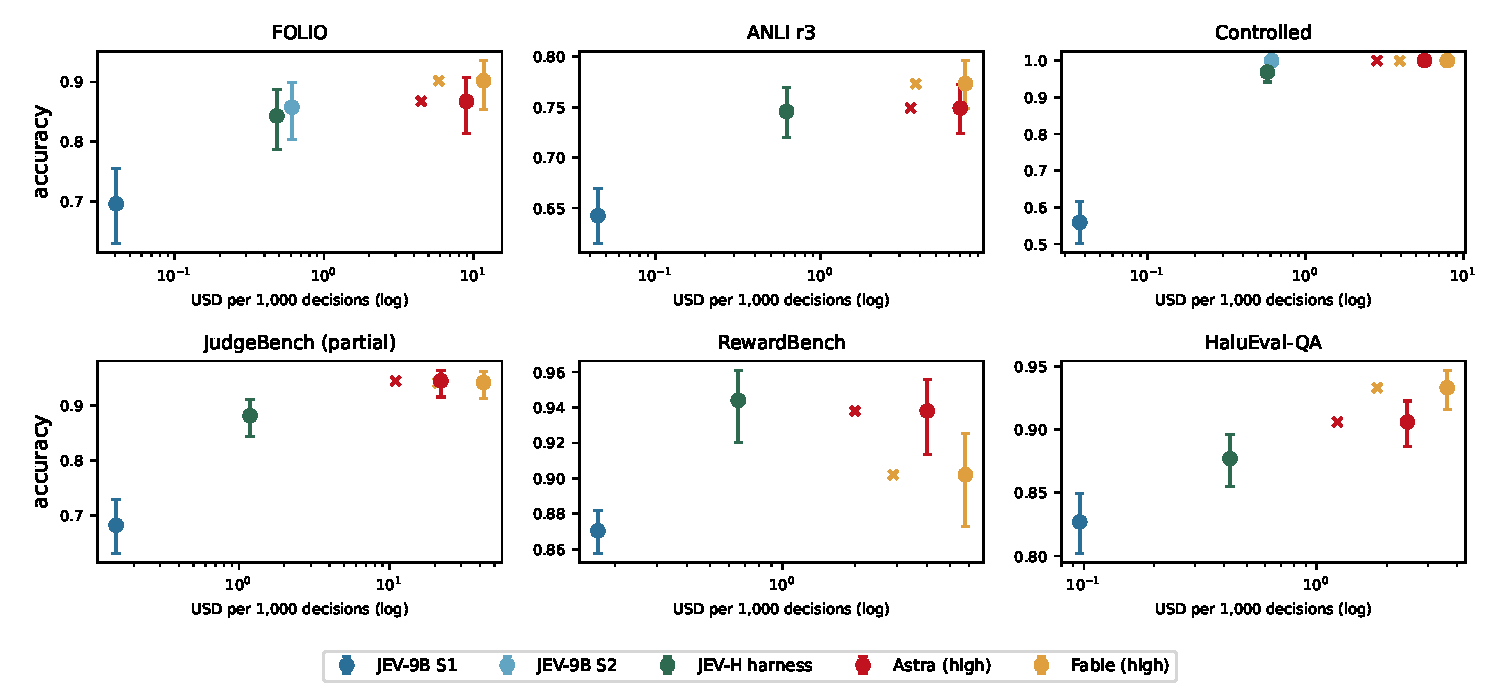
\includegraphics[width=\linewidth]{figures/operating_points.pdf}
\caption{Accuracy (95\% Wilson interval) against cost per 1{,}000 decisions (log scale). Circles: measured synchronous list price; crosses: the same frontier usage at batch prices. JEV-9B sits 25--290 times to the left of both frontiers.}
\label{fig:op}
\end{figure}

\subsection{Public reasoning panels: the frontiers are materially more accurate}
\label{sec:public}
On both primary panels the frozen rule returns \emph{frontier materially more accurate} against both providers (Table~\ref{tab:paired}).
On FOLIO, JEV-9B System~1 is correct on \AccFolioSone\% of items against \AccFolioAstra\% for Astra and \AccFolioFable\% for Fable ($\Delta=\DeltaFolioAstra$ and $\DeltaFolioFable$ points; adjusted upper bounds \HiFolioAstra{} and \HiFolioFable{}).
On ANLI round 3 the gaps are \DeltaAnliAstra{} and \DeltaAnliFable{} points, with upper bounds of \HiAnliAstra{} and \HiAnliFable{}: even the most favourable end of each interval is far outside the two-point margin.
The cost difference runs the other way by a similar order: \$\CostFolioSone{} per thousand FOLIO decisions for JEV-9B against \$\CostFolioAstra{} and \$\CostFolioFable{} for the frontiers.
Neither frontier was close to its output budget: mean output, including reasoning, was 49--137 tokens per item at \texttt{high} effort.

\paragraph{The same weights, thinking, close most of the gap.}
JEV-9B System~2---the identical backbone with its reasoning enabled---reaches \AccFolioStwo\% on FOLIO, within a point of Astra (\AccFolioAstra\%), at \$\CostFolioStwo{} per thousand decisions (Table~\ref{tab:main}).
The deficit of the one-pass decision path is therefore not a deficit of the backbone's knowledge: the information needed is in the weights, and a single forward pass does not extract it.

\subsection{The controlled panel: not depth, but the absence of a derivation}
\label{sec:controlled-results}
\begin{table}[t]
\centering\small
\caption{Controlled panel accuracy (\%) by dependency depth $d$ and irrelevant facts $c$ (48 seeds per cell), and by gold label (96 items each). Chance is 33\%.}
\label{tab:cells}
\begin{tabular}{@{}lcccccc|ccc@{}}
\toprule
& \multicolumn{2}{c}{$d=1$} & \multicolumn{2}{c}{$d=3$} & \multicolumn{2}{c|}{$d=5$} & \multicolumn{3}{c}{Gold label} \\
System & $c{=}0$ & $c{=}8$ & $c{=}0$ & $c{=}8$ & $c{=}0$ & $c{=}8$ & True & False & Unk. \\
\midrule
JEV-9B S1 & 60 & 62 & 60 & 40 & 67 & 46 & 62 & 80 & 25 \\
JEV-9B S2 & 100 & 100 & 100 & 100 & 100 & 100 & 100 & 100 & 100 \\
JEV-H harness & 98 & 98 & 94 & 98 & 96 & 98 & 99 & 98 & 94 \\
Astra (high) & 100 & 100 & 100 & 100 & 100 & 100 & 100 & 100 & 100 \\
Fable (high) & 100 & 100 & 100 & 100 & 100 & 100 & 100 & 100 & 100 \\
\bottomrule
\end{tabular}
\end{table}

\begin{table}[t]
\centering\small
\caption{Depth and distractor interactions on the controlled panel (points). $\Delta_J$, $\Delta_F$: change in JEV-9B~S1 and comparator accuracy between levels; DID $=\Delta_J-\Delta_F$. H1: Bonferroni $\alpha=0.05/6$; H1c (same-weights System~2 comparator): $\alpha=0.05$. Cluster bootstrap over 48 seeds. \checkmark: interval excludes 0.}
\label{tab:did}
\begin{tabular}{@{}lllrrrcc@{}}
\toprule
Fam. & Comparator & Contrast & $\Delta_J$ & $\Delta_F$ & DID & Adj.\ CI & \\
\midrule
H1 & Astra (high) & depth 5 vs 1 & -5.2 & 0.0 & -5.2 & [-24.0, 13.5] &  \\
H1 & Astra (high) & depth 3 vs 1 & -11.5 & 0.0 & -11.5 & [-28.1, 6.2] &  \\
H1 & Astra (high) & distractors 8 vs 0 & -13.2 & 0.0 & -13.2 & [-27.1, 0.7] &  \\
H1 & Fable (high) & depth 5 vs 1 & -5.2 & 0.0 & -5.2 & [-24.0, 13.5] &  \\
H1 & Fable (high) & depth 3 vs 1 & -11.5 & 0.0 & -11.5 & [-28.1, 6.2] &  \\
H1 & Fable (high) & distractors 8 vs 0 & -13.2 & 0.0 & -13.2 & [-27.1, 0.7] &  \\
H1c & JEV-9B S2 & depth 5 vs 1 & -5.2 & 0.0 & -5.2 & [-18.8, 8.3] &  \\
H1c & JEV-9B S2 & depth 3 vs 1 & -11.5 & 0.0 & -11.5 & [-24.0, 1.0] &  \\
\bottomrule
\end{tabular}
\end{table}

\begin{table}[t]
\centering\small
\caption{Paired controls at $d{=}3$, $c{=}8$ (48 seeds, \%). Changing: one verified edit flips the gold label. Preserving: renamed entities and reordered premises, same label. ``Changed'' = answer differs from the base answer; ``Both'' = correct on base and edited item; ``Invariant'' = same answer as base.}
\label{tab:controls}
\begin{tabular}{@{}lrrrrrr@{}}
\toprule
& Base & \multicolumn{3}{c}{Decision-changing} & \multicolumn{2}{c}{Decision-preserving} \\
System & acc. & acc. & changed & both & acc. & invariant \\
\midrule
JEV-9B S1 & 40 & 58 & 48 & 23 & 31 & 58 \\
JEV-9B S2 & 100 & 100 & 100 & 100 & 100 & 100 \\
JEV-H harness & 98 & 98 & 98 & 96 & 98 & 96 \\
Astra (high) & 100 & 100 & 100 & 100 & 100 & 100 \\
Fable (high) & 100 & 100 & 100 & 100 & 100 & 100 \\
\bottomrule
\end{tabular}
\end{table}


Every reasoning system---both frontiers and JEV-9B System~2---answers all 288 base items correctly at every depth and context (Table~\ref{tab:cells}); the fragment is easy for any system that reasons.
JEV-9B System~1 is correct on \AccCtlSone\%.
Our primary hypothesis H1 predicted that this deficit would grow with dependency depth.
\textbf{It did not, at our precision.}
Moving from depth~1 to depth~5 changes System~1 accuracy by \ChgAstraDfive{} points, a difference-in-differences of \DidAstraDfive{} against either frontier with an adjusted interval of [\DidLoAstraDfive, \DidHiAstraDfive] (Table~\ref{tab:did}); depth~3 gives \DidAstraDthree{} [\DidLoAstraDthree, \DidHiAstraDthree].
Neither interval excludes zero, so H1 is not supported; with 48 seeds we cannot exclude a moderate depth effect either.
The eight irrelevant facts, which add about 250 characters, move accuracy by \DidAstraCtx{} points [\DidLoAstraCtx, \DidHiAstraCtx]---a larger point estimate than depth, contrary to H1b, though its interval also touches zero.

The structure of the errors is clearer than their dependence on depth.
By gold label (Table~\ref{tab:cells}, right), System~1 is correct on most \emph{False} items and on a majority of \emph{True} items, but on only a quarter of \emph{Unknown} items: it rarely concludes that nothing follows.
Its predictions are also unstable under edits that should not matter: renaming entities and reordering premises preserves its answer on only \CtlSoneInvariant\% of seeds, against 100\% for every reasoning system (Table~\ref{tab:controls}).
And under an edit that flips the verified label, it changes its answer on \CtlSoneAnswerChanged\% of seeds and is right on both the original and the edited item on only \CtlSoneBothCorrect\%.
Together these say that, on this fragment, the one-pass model is not tracking the derivation at all: it reads surface cues, and the cue it most lacks is the one for ``no rule applies''.

The deep extension (A1; 12 rules, depths 1/5/9, exploratory) shows the same picture with more room: System~1 scores \DeepSoneDOne\%, \DeepSoneDFive\% and \DeepSoneDNine\% at depths 1, 5 and 9, System~2 \DeepStwoDOne\%, \DeepStwoDFive\% and \DeepStwoDNine\%, and both frontiers 100\% throughout (Figure~\ref{fig:depth}).
Even at nine dependent steps the frontier models do not drop an item; whatever their depth limit is, it lies beyond what a 12-rule, sub-1{,}000-character problem can probe.

\begin{figure}[t]
\centering
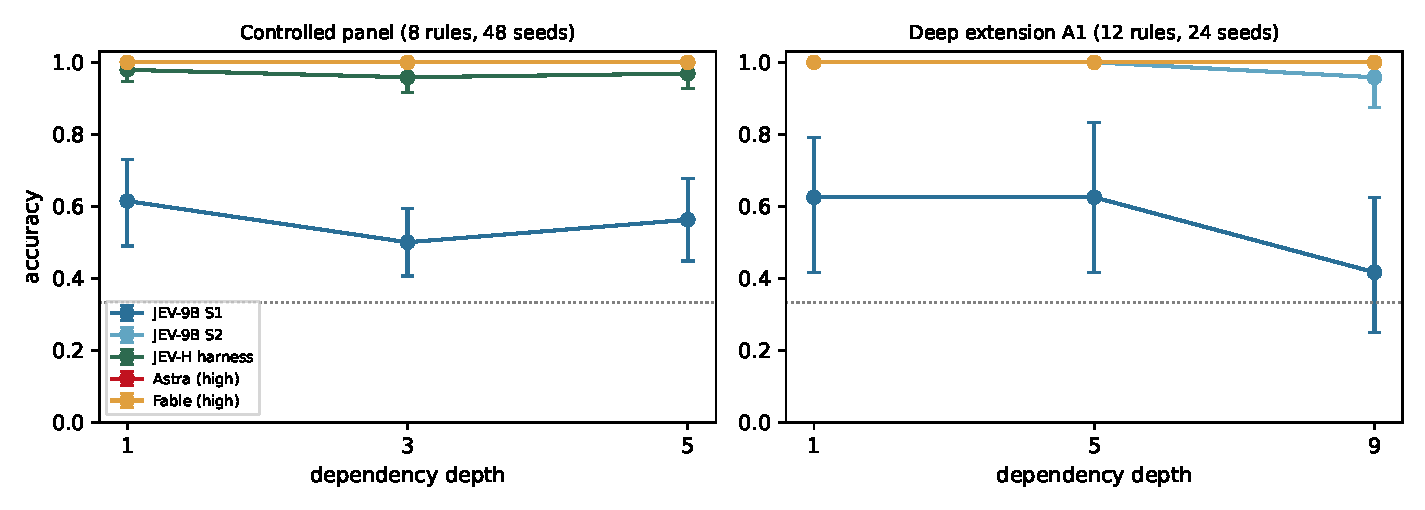
\includegraphics[width=\linewidth]{figures/depth.pdf}
\caption{Accuracy by dependency depth with seed-clustered 95\% bootstrap intervals. Left: the preregistered controlled panel (8 rules, depths 1/3/5). Right: the exploratory deep extension (12 rules, depths 1/5/9). Dotted line: chance.}
\label{fig:depth}
\end{figure}

\paragraph{Same weights, different computation (H1c).}
Against its own System~2, System~1's depth-3-versus-depth-1 difference-in-differences is \DidStwoDthree{} points [\DidLoStwoDthree, \DidHiStwoDthree] and depth-5-versus-1 is \DidStwoDfive{} [\DidLoStwoDfive, \DidHiStwoDfive].
Because System~2 is flat at 100\%, these contrasts mostly restate System~1's own variation; the more informative statement is the level: identical weights solve every controlled item when allowed to reason, and solve \AccCtlSone\% when not.

\subsection{Judging LLM outputs}
\label{sec:judging}
\begin{table}[t]
\centering\small
\caption{RewardBench (2{,}985 filtered pairs) accuracy (\%) by official section; ``Score'' is the unweighted section mean, ``All'' the item mean. HaluEval-QA answer-length-only AUROC (trivial baseline): 0.976.}
\label{tab:judgetrack}
\begin{tabular}{@{}lrrrrrr@{}}
\toprule
System & Chat & Chat Hard & Safety & Reasoning & Score & All \\
\midrule
JEV-9B S1 & 96.4 & 67.5 & 90.1 & 89.3 & 85.8 & 87.0 \\
JEV-9B S2 & 81.8 & 83.7 & 87.2 & 98.6 & 87.8 & 92.2 \\
JEV-H harness & 93.3 & 81.7 & 94.0 & 98.7 & 91.9 & 94.4 \\
Astra (high) & 86.7 & 84.5 & 91.0 & 100.0 & 90.5 & 93.8 \\
Fable (high) & 96.7 & 87.3 & 71.4 & 100.0 & 88.9 & 90.2 \\
\bottomrule
\end{tabular}
\end{table}

\begin{table}[t]
\centering\small
\caption{Accuracy (\%) on inputs of at most / more than 1{,}024 JEV-9B tokens, the length on which JEV-9B was trained. Only panels with long inputs are shown.}
\label{tab:length}
\begin{tabular}{@{}lcccccc@{}}
\toprule
Panel & $n$ short/long & JEV-9B S1 & JEV-9B S2 & JEV-H & Astra & Fable \\
\midrule
JudgeBench (partial) & 54 / 292 & 64.8 / 68.8 & 73.5 / 87.9 & 87.0 / 88.4 & 88.9 / 95.5 & 94.4 / 94.2 \\
RewardBench & 2778 / 206 & 87.2 / 85.0 & 92.4 / 89.5 & 94.3 / 96.4 & 93.9 / 92.9 & 89.8 / 96.4 \\
\bottomrule
\end{tabular}
\end{table}


The judge track asks whether JEV-9B can replace a frontier LLM-as-a-judge.
\textbf{On RewardBench it is the closest to parity of any panel.}
One-pass JEV-9B is correct on \AccRbSone\% of all 2{,}985 filtered pairs; on the sealed 500-pair sample shared with the frontiers it trails Astra by \DeltaRbAstra{} points [\LoRbAstra, \HiRbAstra] and Fable by only \DeltaRbFable{} points [\LoRbFable, \HiRbFable] (Table~\ref{tab:paired}).
Against Fable the interval includes zero but not the full two-point margin, so the frozen rule returns \emph{inconclusive}: we can neither certify noninferiority nor show a difference.
By section (Table~\ref{tab:judgetrack}), JEV-9B matches Fable on Chat (\RbSoneChat\% vs.\ \RbFableChat\%) and \emph{exceeds} it on Safety (\RbSoneSafety\% vs.\ \RbFableSafety\%), where Fable's refusals to adjudicate harmful prompts count against it; it is clearly weaker on Chat Hard (\RbSoneChatHard\% vs.\ \RbFableChatHard\%), the adversarial instruction-following pairs, and on Reasoning (\RbSoneReasoning\% vs.\ 100\%).
It does this at \$\CostRbSone{} per thousand judgements, against \$\CostRbAstra{} and \$\CostRbFable.

On JudgeBench---difficult, mostly long correctness judgements---the gap is large (\DeltaJbgptAstra{} and \DeltaJbgptFable{} points on the GPT-response split; the Claude split has too few completed rows to analyse, Appendix~\ref{app:prereg}).
On HaluEval-QA JEV-9B detects hallucinated answers at \AccHaluSone\%, against \AccHaluAstra\% and \AccHaluFable\% (gaps \DeltaHaluAstra{} and \DeltaHaluFable).
\emph{All three judges are below a trivial baseline here}: answer length alone separates right from hallucinated answers with AUROC \HaluLenAuroc, because HaluEval's hallucinated answers are systematically longer.
We report HaluEval for completeness but draw no conclusion about hallucination detection from it.



\subsection{Is the one-pass probability calibrated?}
\label{sec:calibration}
\begin{table}[t]
\centering\small
\caption{Calibration of JEV-9B System~1's top probability by task family: mean confidence, accuracy, their gap (overconfidence, points) and expected calibration error (15 bins).}
\label{tab:calibration}
\begin{tabular}{@{}lrrrrr@{}}
\toprule
Family & $n$ & Mean conf. & Accuracy & Over-conf. & ECE \\
\midrule
anli & 1200 & 73.0 & 64.2 & 8.8 & 0.105 \\
controlled & 488 & 66.9 & 56.1 & 10.7 & 0.116 \\
folio & 204 & 76.4 & 69.6 & 6.8 & 0.098 \\
halueval & 1000 & 89.0 & 82.7 & 6.3 & 0.067 \\
judgebench & 349 & 75.5 & 68.2 & 7.3 & 0.085 \\
rewardbench & 2984 & 88.5 & 87.0 & 1.5 & 0.026 \\
\bottomrule
\end{tabular}
\end{table}

\begin{figure}[t]
\centering
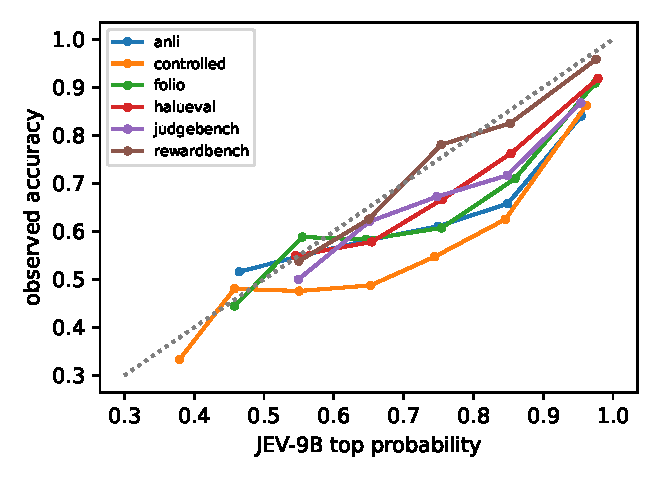
\includegraphics[width=0.55\linewidth]{figures/calibration.pdf}
\caption{Reliability of JEV-9B System~1's top probability by task family (bins with at least 15 items).}
\label{fig:calibration}
\end{figure}
A decision model's selling point is its probability, so we test it out of distribution (Table~\ref{tab:calibration}, Figure~\ref{fig:calibration}).
On RewardBench the top probability is well calibrated (mean confidence 88.5\% against 87.0\% accuracy; ECE 0.026).
On the reasoning panels it is systematically overconfident by 6.8 (FOLIO) to 10.7 (controlled) points, with ECE around 0.10---two orders of magnitude above the 0.0007 the model card reports on its in-distribution test set.
Confidence remains informative for ranking (it is what makes the JEV-H gate work), but a deployment should not read a 0.8 from JEV-9B on a reasoning task as an 80\% chance of being right without recalibrating on its own data.

\subsection{The JEV-H harness}
\label{sec:harness-results}
\begin{table*}[t]
\centering\small
\caption{JEV-H harness (A4: two option orders, threshold 0.90 fixed a priori, escalation to JEV-9B's own System~2) against each frontier. $\Delta$ = JEV-H minus frontier (points); intervals Bonferroni-adjusted over all 12 panel $\times$ frontier pairs. $^\dagger$Not preregistered: all 25 of Claude Fable's RewardBench refusals are Safety pairs, scored incorrect in the primary row; this row drops them.}
\label{tab:harness}
\resizebox{\linewidth}{!}{\begin{tabular}{@{}llrrrcl@{}}
\toprule
Panel & Frontier & JEV-H & Frontier & $\Delta$ & Adj.\ CI & Conclusion \\
\midrule
FOLIO & Astra (high) & 84.3 & 86.8 & -2.5 & [-9.6, 5.1] & inconclusive \\
 & Fable (high) & 84.3 & 90.2 & -5.9 & [-12.9, 0.0] & inconclusive \\
ANLI r3 & Astra (high) & 74.6 & 74.9 & -0.3 & [-3.9, 3.1] & inconclusive \\
 & Fable (high) & 74.6 & 77.3 & -2.8 & [-6.1, 0.6] & inconclusive \\
Controlled & Astra (high) & 96.9 & 100.0 & -3.1 & [-6.2, -0.7] & inconclusive \\
 & Fable (high) & 96.9 & 100.0 & -3.1 & [-6.2, -0.7] & inconclusive \\
JudgeBench (partial) & Astra (high) & 88.2 & 94.5 & -6.4 & [-19.1, -1.5] & inconclusive \\
 & Fable (high) & 88.2 & 94.2 & -6.1 & [-16.6, -1.9] & inconclusive \\
RewardBench & Astra (high) & 94.4 & 93.8 & 0.6 & [-2.4, 3.6] & inconclusive \\
 & Fable (high) & 94.4 & 90.2 & 4.2 & [0.4, 8.2] & JEV-H better \\
HaluEval-QA & Astra (high) & 87.7 & 90.6 & -2.9 & [-5.3, -0.7] & inconclusive \\
 & Fable (high) & 87.7 & 93.3 & -5.6 & [-8.2, -3.3] & frontier better \\
\addlinespace
RewardBench, refusals excluded$^\dagger$ & Fable (high) & 94.1 & 94.9 & -0.8 & [-4.0, 2.1] & sensitivity only ($n=475$) \\
\bottomrule
\end{tabular}}
\end{table*}


JEV-H (preregistration A4) asks System~1 in both option orders and escalates to System~2 when the averaged confidence is below 0.90; it has no fitted parameter.
Its escalation rate is itself informative: \EscHalueval\% of HaluEval, \EscRewardbench\% of RewardBench, \EscFolio\% of FOLIO, \EscAnli\% of ANLI and \EscJudgebench\% of JudgeBench items fall below the threshold, so the one-pass model is confident mostly where it is accurate.
Table~\ref{tab:harness} compares the harness with each frontier in its own Bonferroni family of 12 comparisons.

\textbf{On RewardBench the harness is the most accurate system we tested.}
It is correct on \AccRbHarn\% of the 500 shared pairs, against \AccRbAstra\% for Astra ($\Delta=\DeltaHRbAstra$ [\LoHRbAstra, \HiHRbAstra]) and \AccRbFable\% for Fable ($\Delta=\DeltaHRbFable$ [\LoHRbFable, \HiHRbFable]).
Under the preregistered scoring the frozen rule returns \emph{\ConclHRbFable} against Fable.
That verdict needs one qualification, which we state as prominently as the result: all 25 of Fable's refusals are Safety pairs, scored as errors.
On the 475 pairs Fable answered, JEV-H and Fable are statistically indistinguishable (\AccHRbFableAnsweredH\% vs.\ \AccHRbFableAnsweredF\%, $\Delta=\DeltaHRbFableAnswered$ [\LoHRbFableAnswered, \HiHRbFableAnswered]; a sensitivity analysis that was not preregistered).
Against Astra the interval sits within $[-2.4, 3.6]$: the harness neither loses nor certifiably matches it under the two-point margin.
It does this at \$\CostRbHarn{} per thousand judgements, against \$\CostRbAstra{} and \$\CostRbFable.

On the reasoning panels the harness recovers most of the one-pass deficit.
On ANLI it is \AccAnliHarn\% against Astra's \AccAnliAstra\% ($\Delta=\DeltaHAnliAstra$ [\LoHAnliAstra, \HiHAnliAstra]), up from System~1's \AccAnliSone\%; on FOLIO \AccFolioHarn\% against \AccFolioAstra\%; on the controlled panel \AccCtlHarn\%.
None of these reach the frozen rule's \emph{comparable} verdict---their lower bounds pass the two-point margin---but none is a material frontier advantage either, where System~1 alone was.
The harness still trails clearly on HaluEval (\AccHaluHarn\% vs.\ \AccHaluFable\% for Fable) and on JudgeBench (\AccJbgptHarn\% vs.\ \AccJbgptAstra\%), the two panels whose judgements need factual verification of long answers.
Its cost is \$\CostFolioHarn--\$\CostJbgptHarn{} per thousand items, 6--35 times cheaper than the frontier on the same panel, even with System~2 charged conservatively for all pod time (Table~\ref{tab:main}).


\paragraph{Threshold sensitivity (exploratory).}
\begin{figure}[t]
\centering
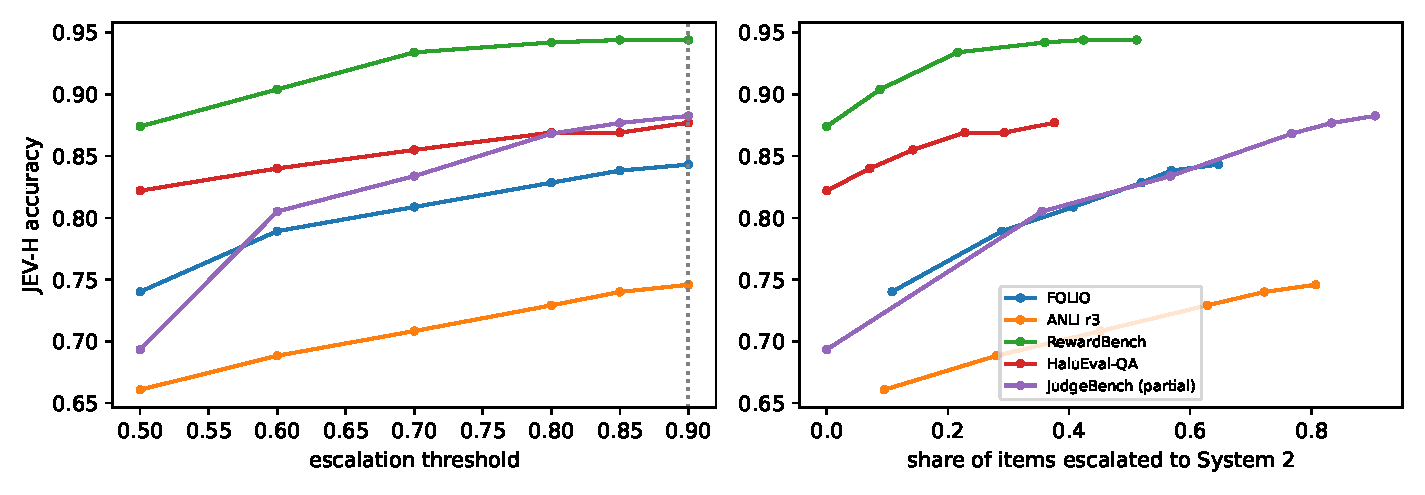
\includegraphics[width=\linewidth]{figures/threshold.pdf}
\caption{JEV-H as the escalation threshold varies (exploratory; the preregistered threshold is 0.90, dotted). Left: accuracy against threshold. Right: accuracy against the share of items escalated to System~2.}
\label{fig:threshold}
\end{figure}
The preregistered threshold of 0.90 was fixed a priori; Figure~\ref{fig:threshold} shows what lower thresholds would have bought, using the System~2 answers already collected.
Most of the gain arrives early: on RewardBench a threshold of 0.70 reaches 93.4\% while escalating 22\% of items (0.90: 94.4\% at 51\%), and on JudgeBench 0.60 already lifts accuracy from 69.3\% to 80.5\% at 36\% escalation.
On FOLIO and ANLI the curve keeps rising to 0.90, because the one-pass model is unsure on most items.
A deployment should choose its threshold from this curve on its own labelled data; \texttt{jevstudy judge} reports it.

\subsection{Robustness}
\label{sec:robust}
\begin{table}[t]
\centering\small
\caption{Option-order reversal (all systems see the reversed list). Flip rate: share of items whose answer, mapped back to the original order, differs from the original answer (\%).}
\label{tab:reversal}
\begin{tabular}{@{}llrrrr@{}}
\toprule
Panel & System & $n$ & Acc.\ orig. & Acc.\ rev. & Flip rate \\
\midrule
FOLIO & JEV-9B S1 & 204 & 69.6 & 68.1 & 5.9 \\
\addlinespace
Controlled base & JEV-9B S1 & 288 & 55.9 & 55.6 & 3.5 \\
\bottomrule
\end{tabular}
\end{table}

Reversing the option list changes System~1's answer on \FlipFolioSone\% of FOLIO items and \FlipCtlSone\% of controlled items (Table~\ref{tab:reversal}), well below the 11.5\% the model card reports for sixteen-option lists; on these three-option tasks position bias is not the main error source.
The frontier arms of this ablation and the max-effort ablation were dropped to limit spending (A5).

\subsection{Can pre-call features say when JEV-9B is enough?}
\label{sec:routing-results}
\begin{table*}[t]
\centering\small
\caption{Selection rules (H3). Leave-one-family-out over five families: mean held-out accuracy (\%), number of folds within 2 points of always-frontier, share of items sent to JEV-9B (\%), and total cost relative to always-frontier. Unseen template: rules fit on everything except controlled template T2, evaluated on T2 items.}
\label{tab:routing}
\begin{tabular}{@{}llrrrrrr@{}}
\toprule
& & \multicolumn{4}{c}{Leave one family out} & \multicolumn{2}{c}{Unseen template T2} \\
Frontier & Policy & Acc. & Within 2 pt & To JEV & Cost ratio & Acc. & To JEV \\
\midrule
Astra & Always JEV-9B & 71.5 & 0/6 & 100 & 0.01 & 49.3 & 100 \\
 & Always frontier & 90.1 & 6/6 & 0 & 1.00 & 100.0 & 0 \\
 & Length only & 90.1 & 6/6 & 1 & 1.00 & 100.0 & 0 \\
 & Family lookup & 90.1 & 6/6 & 0 & 1.00 & 100.0 & 0 \\
 & JEV-9B confidence gate & 87.6 & 4/6 & 45 & 0.67 & 95.1 & 26 \\
 & Feature rule & 87.7 & 4/6 & 19 & 0.84 & 100.0 & 0 \\
 & Feature rule + conf. & 89.3 & 4/6 & 17 & 0.88 & 100.0 & 0 \\
 & Oracle (unattainable) & 93.4 & 6/6 & 78 & 0.25 & 100.0 & 49 \\
\midrule
Fable & Always JEV-9B & 71.5 & 1/6 & 100 & 0.01 & 49.3 & 100 \\
 & Always frontier & 90.9 & 6/6 & 0 & 1.00 & 100.0 & 0 \\
 & Length only & 90.9 & 6/6 & 0 & 1.00 & 100.0 & 0 \\
 & Family lookup & 90.9 & 6/6 & 0 & 1.00 & 100.0 & 0 \\
 & JEV-9B confidence gate & 88.5 & 1/6 & 45 & 0.66 & 95.1 & 26 \\
 & Feature rule & 87.0 & 4/6 & 23 & 0.74 & 100.0 & 0 \\
 & Feature rule + conf. & 88.6 & 4/6 & 21 & 0.78 & 100.0 & 0 \\
 & Oracle (unattainable) & 94.3 & 6/6 & 77 & 0.27 & 100.0 & 49 \\
\bottomrule
\end{tabular}
\end{table*}

Under leave-one-family-out evaluation (Table~\ref{tab:routing}), no rule reaches the always-frontier accuracy band on every held-out family.
Against Astra, the JEV-9B confidence gate keeps \RouteAstraGateAcc\% mean held-out accuracy (always-Astra: \RouteAstraAfrAcc\%) at \RouteAstraGateCost{} of the cost, and is within two points of always-Astra on \RouteAstraGateWithin{} folds; the feature rule plus confidence reaches \RouteAstraRuleconfAcc\% at \RouteAstraRuleconfCost{} of the cost (\RouteAstraRuleconfWithin{} folds).
Length-only and family-lookup rules degenerate to always-frontier on held-out families.
H3 is therefore only partly supported: features add a little to the confidence gate, neither reliably preserves frontier accuracy on a family it was not fit on, and the oracle (\RouteAstraOracleAcc\% at \RouteAstraOracleCost{} of the cost) shows how much routing headroom remains.

\subsection{Bridge to official Jev}
\label{sec:bridge}
\begin{table}[t]
\centering\small
\caption{ProofWriter bridge (A2, exploratory). JEV-9B~S1 accuracy (\%) on 900 open-world items (50 per depth $\times$ label) with Hard-Decisions' task wording, beside official Jev, Kev-9B and GPT-6 Luna (reasoning off) as published by Hard-Decisions on a different sample of the same strata. JEV-9B by label: true 54.2, false 57.3, unknown 71.1.}
\label{tab:bridge}
\begin{tabular}{@{}rrrcrrr@{}}
\toprule
Depth & $n$ & JEV-9B S1 & 95\% CI & Official Jev & Kev-9B & Luna (off) \\
\midrule
0 & 150 & 94.0 & [89.0, 96.8] & 97.7 & 89.3 & 93.3 \\
1 & 150 & 72.7 & [65.0, 79.2] & 87.7 & 73.8 & 77.8 \\
2 & 150 & 57.3 & [49.3, 65.0] & 84.8 & 58.4 & 60.4 \\
3 & 148 & 56.8 & [48.7, 64.5] & 79.9 & 49.5 & 61.7 \\
4 & 149 & 42.3 & [34.6, 50.3] & 71.9 & 38.6 & 44.6 \\
5 & 143 & 40.6 & [32.9, 48.8] & 81.0 & 41.2 & 46.0 \\
\bottomrule
\end{tabular}
\end{table}

\begin{figure}[t]
\centering
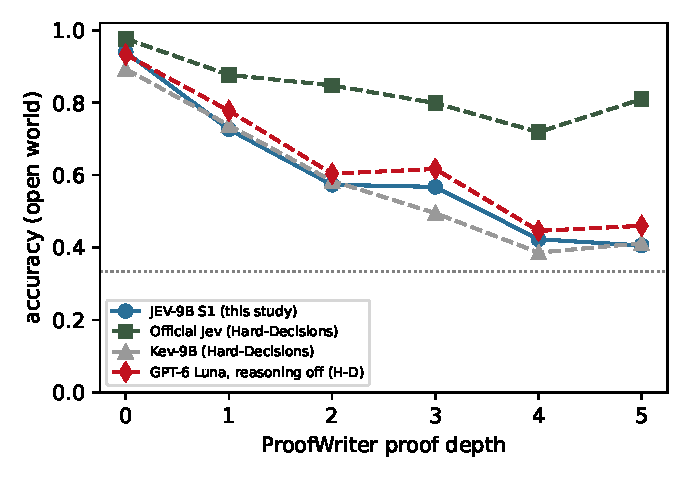
\includegraphics[width=0.62\linewidth]{figures/bridge.pdf}
\caption{ProofWriter open-world accuracy by proof depth: JEV-9B~S1 (this study, 900 items) against official Jev, Kev-9B and GPT-6 Luna without reasoning as published by Hard-Decisions on a different sample of the same strata.}
\label{fig:bridge}
\end{figure}
On ProofWriter (A2, exploratory), JEV-9B falls from \BridgeDZero\% at depth~0 to \BridgeDFive\% at depth~5 (Table~\ref{tab:bridge}, Figure~\ref{fig:bridge}).
Official Jev, on a different sample of the same strata, falls only to 81.0\%.
At depth~0 the student is within four points of its teacher; from depth~2 on it tracks Kev-9B, a different 9B decision model, and not Jev.
\textbf{This is the most important qualification of everything above}: the student's reasoning-depth behaviour is not the teacher's, so our negative results about JEV-9B on reasoning panels should not be read as results about official Jev.

\FloatBarrier
\section{Discussion}
\label{sec:discussion}

\paragraph{When can a decision model replace a reasoning LLM?}
Table~\ref{tab:scorecard} collects the verdicts.
On the evidence here, JEV-9B is not a replacement for a frontier model on tasks whose answer must be \emph{derived}: natural-language deduction, adversarial inference and hard correctness judgements all show materially lower accuracy, and the controlled panel shows that the failure is present even when the derivation is a single rule.
It is closest to a replacement where the judgement is \emph{recognitional}---whether a chat response is the helpful one, whether a response appropriately handles a harmful request---as on RewardBench's Chat and Safety sections.
And it is 25--290 times cheaper on every panel (25--38$\times$ on the judge track, where frontier calls are shortest), with a calibrated probability that a deployment can threshold.

\paragraph{What the same-weights arm adds.}
Most comparisons between decision models and frontier models confound three things: one forward pass versus reasoning, a 9B backbone versus a frontier one, and different training data.
Holding the weights fixed removes the second and third.
JEV-9B's backbone, allowed to think, matches GPT-6 Astra on FOLIO and solves the controlled panel; allowed one pass, it does neither.
For practitioners this suggests a cheaper escalation target than a frontier API---the model's own reasoning mode on the same GPU---and JEV-H shows it works: escalating the 38--91\% of items on which the one-pass model is unsure lifts RewardBench to \AccRbHarn\% and ANLI to \AccAnliHarn\%, at 6--35 times lower cost than a frontier judge.

\paragraph{Why depth did not matter.}
We expected the one-pass model to degrade with each additional dependent step, as models without reasoning do on ProofWriter~\citep{harddecisions2026}.
On our fragment, it was already far from ceiling at depth one, and its errors were dominated by a reluctance to answer \emph{Unknown} and by instability under renaming and reordering.
One reading is that a one-pass reader of an unfamiliar formal fragment does not follow rule chains at all, so their length is irrelevant; on ProofWriter, whose natural vocabulary it saw in distillation, depth does matter (Appendix Table~\ref{tab:bridge}).
A depth effect may therefore require familiarity with the surface form before it can appear.


\paragraph{When is the frontier worth paying for?}
\begin{table}[t]
\centering\small
\caption{Break-even cost of one error. With expected loss $=$ cost per decision $+$ $P(\text{error})\times c$, paying for the frontier instead of the JEV-9B configuration is worth it only when an error costs more than $c^*=\Delta\text{cost}/\Delta\text{accuracy}$. ``never'': the JEV-9B configuration is at least as accurate and cheaper.}
\label{tab:breakeven}
\begin{tabular}{@{}llrr@{}}
\toprule
Panel & Cheap system & $c^*$ vs.\ Astra & $c^*$ vs.\ Fable \\
\midrule
FOLIO & JEV-9B S1 & \$0.052 & \$0.057 \\
 & JEV-H harness & \$0.346 & \$0.190 \\
ANLI r3 & JEV-9B S1 & \$0.065 & \$0.057 \\
 & JEV-H harness & \$1.91 & \$0.251 \\
Controlled & JEV-9B S1 & \$0.013 & \$0.018 \\
 & JEV-H harness & \$0.162 & \$0.233 \\
JudgeBench (partial) & JEV-9B S1 & \$0.083 & \$0.162 \\
 & JEV-H harness & \$0.327 & \$0.677 \\
RewardBench & JEV-9B S1 & \$0.057 & \$0.177 \\
 & JEV-H harness & never & never \\
HaluEval-QA & JEV-9B S1 & \$0.030 & \$0.033 \\
 & JEV-H harness & \$0.070 & \$0.057 \\
\bottomrule
\end{tabular}
\end{table}

Expected loss per decision is its cost plus the probability of an error times what an error costs; paying for the frontier is worth it exactly when an error costs more than $c^*=\Delta\text{cost}/\Delta\text{accuracy}$ (Table~\ref{tab:breakeven}).
Against one-pass JEV-9B, $c^*$ is between one and eighteen cents on every panel: whenever a wrong decision costs a user more than a few cents---a mislabelled support ticket, an accepted bad answer in an evaluation set---the frontier's accuracy pays for itself.
JEV-H raises $c^*$ by 2--30$\times$ (HaluEval to ANLI), and on RewardBench to \emph{never}: there the harness is both more accurate and cheaper than either frontier.
The decision rule is established decision analysis, not a contribution; the measured inputs to it are.

\paragraph{Cost, measured.}
At high effort both frontier models reasoned briefly---tens to a few hundred output tokens per item---so the frontier cost per decision was \$0.002--0.04, far below the planning estimates.
The economic case for a decision model is thus not that frontier reasoning is unaffordable, but that it is 25--290 times more expensive per decision, which matters at evaluation volume.
The whole study, including every API call, cost \$\ApiTotal{} in API fees plus a single rented GPU.

\begin{table}[t]
\centering\small
\caption{Scorecard. Each verdict follows the frozen rule against both frontiers unless stated; ``cost'' compares measured cost per 1{,}000 decisions.}
\label{tab:scorecard}
\begin{tabularx}{\linewidth}{@{}p{0.34\linewidth}Xp{0.17\linewidth}@{}}
\toprule
Question & Evidence & Verdict \\
\midrule
Replace frontier on deduction / NLI? & FOLIO, ANLI: $-11$ to $-21$ points & No \\
Replace frontier as a pairwise judge (one pass)? & RewardBench: $\DeltaRbFable$ vs.\ Fable [\LoRbFable, \HiRbFable], $\DeltaRbAstra$ vs.\ Astra & Inconclusive / close \\
Replace it with the JEV-H harness? & RewardBench \AccRbHarn\% vs.\ \AccRbAstra\%/\AccRbFable\% (tied with Fable without refusals); ANLI $\DeltaHAnliAstra$ & Yes on RewardBench; close on ANLI \\
Replace frontier on hard correctness judging? & JudgeBench: $\approx -26$ points & No \\
Cheaper and faster? & 25--290$\times$ cheaper on every panel & Yes \\
Does depth drive the one-pass deficit (H1)? & DID depth 5 vs.\ 1: \DidAstraDfive{} [\DidLoAstraDfive, \DidHiAstraDfive] & Not supported \\
Is it computation, not knowledge (H1c)? & Same weights with thinking: FOLIO \AccFolioStwo\%, controlled 100\% & Supported \\
Can features predict sufficiency (H3)? & Within 2 pt of frontier on \RouteAstraRuleconfWithin{} held-out folds & Partly \\
Do results transfer to official Jev? & ProofWriter depth 5: \BridgeDFive\% vs.\ 81.0\% & No (student $\neq$ teacher) \\
\bottomrule
\end{tabularx}
\end{table}


\subsection{Threats to validity}
\label{sec:threats}

\paragraph{Construct: a student, not the teacher.}
Every decision-model result is about JEV-9B, a community distillation of Jev~1.13 that its authors report trails the teacher on gold accuracy at every option count, flips 11.5\% of sixteen-option answers under reordering (teacher: 7.0\%), and has a KL of 0.234 on unseen task families.
The ProofWriter bridge (Section~\ref{sec:bridge}) compares the two only at the level of depth-stratified accuracy on different samples of the same strata; it bounds, but does not measure, how far our conclusions transfer to official Jev.

\paragraph{Construct: the controlled fragment.}
The fragment uses unary predicates, single-premise rules and invented words.
It isolates dependency depth from length and vocabulary by construction, at the cost of naturalness; its conclusions apply to this fragment, and the public panels are where naturalness is tested.
Automated round-trip parsing guarantees that each sentence states its formula, but not that a human would read the templates the same way; we could not run the planned blinded human review.

\paragraph{Internal: matched prompts are not matched interfaces.}
All systems see identical task content, but JEV-9B consumes it through a typed template it was trained on, while the frontier models receive free text with a schema-constrained answer.
A prompt engineered separately for each system could change accuracies; we report the common-prompt comparison only, and one-sided prompt tuning would not be a fair alternative.
System~2 answers in free text that we parse; its parse failures are counted as errors.

\paragraph{Internal: provider-side variation.}
Frontier models run on hidden infrastructure whose routing and versions we cannot control; we logged the resolved model on every response and saw no change, but services may differ between the days of our runs.
Reasoning effort names are not comparable compute across providers.

\paragraph{Statistical.}
FOLIO's 204 rows form only 73 independent stories, so its intervals are wide; no FOLIO-only result can certify a two-point margin.
Repeated hypotheses are Bonferroni-adjusted within declared families; exploratory analyses (A1, A2, G02, length strata) carry no multiplicity control and are labelled as such.
Interval coverage was checked by simulation under a latent-normal model, which may not match real discordance structure.

\paragraph{External: cost and latency.}
JEV-9B's cost is GPU time on one rented A40 at one utilisation level; a different card, batch size or utilisation changes it by integer factors.
Frontier prices are dated list prices; negotiated or cached pricing would lower them.
JEV-9B latency excludes a network hop; frontier latency includes one.


\subsection{Limitations}
The decision model is a community student, not TypeSafe Jev; two frontier configurations at one effort level stand for the frontier; the controlled fragment is narrow and was validated automatically rather than by human readers; budget limits reduced RewardBench to 500 pairs and left JudgeBench partial; and HaluEval-QA is solvable by length alone. Section~\ref{sec:threats} discusses threats to validity in full.

\section{Conclusion}
A one-pass decision model is an excellent default for cheap, calibrated, recognitional judgements and a poor substitute for reasoning, and the deficit lives in the computation rather than in the weights: the same weights that fail in one pass succeed when they think.
For evaluation pipelines, that suggests a simple architecture---decision model first, its own reasoning mode or a frontier model only when it is unsure---which on RewardBench matched or exceeded both frontier judges we tested, and a simple discipline: measure, on your own labelled data and with paired intervals, whether the cheap path is good enough before trusting it.
The code, preregistration, item-level predictions and a self-hostable judging API are released at \url{https://github.com/arghya05/jev-boundary-study}.

\FloatBarrier

\bibliographystyle{plainnat}
\bibliography{refs}

\appendix
\section{Additional Analyses}
\label{app:additional}
\begin{figure}[t]
\centering
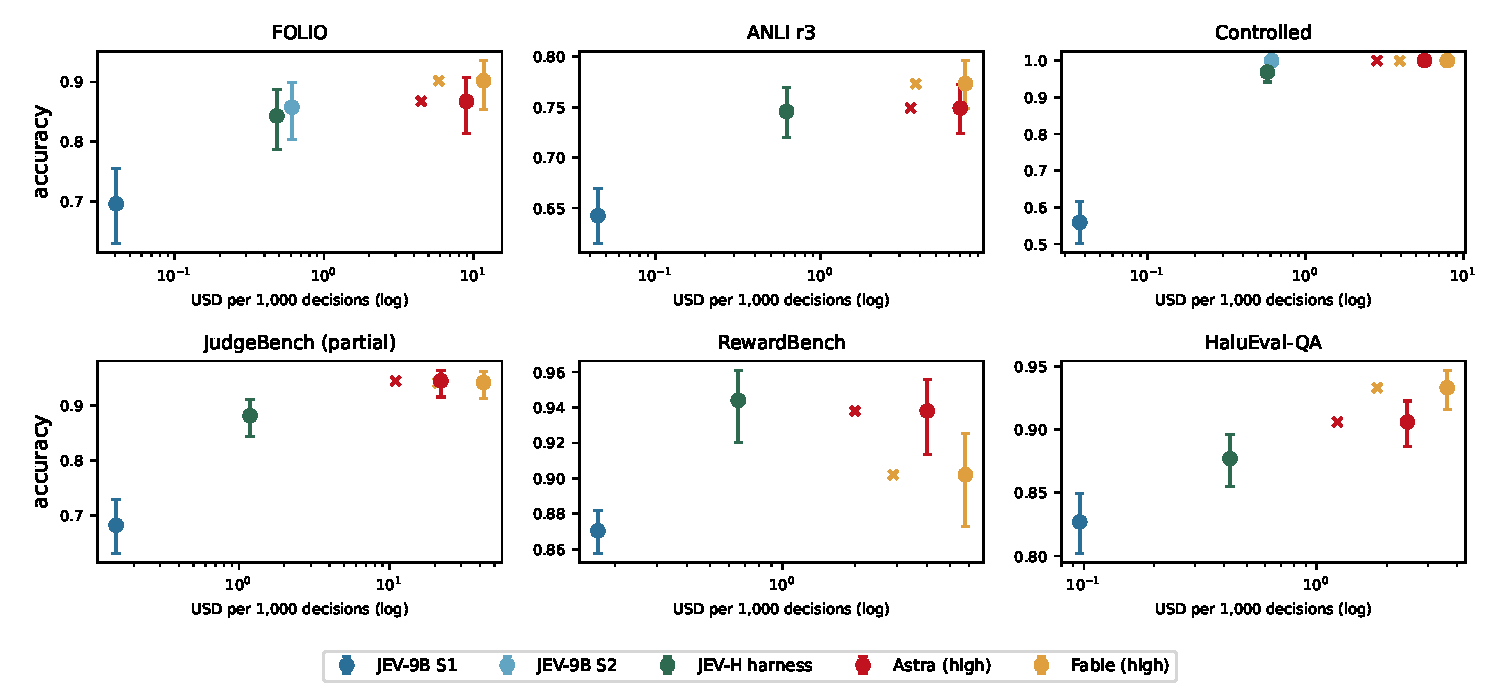
\includegraphics[width=\linewidth]{figures/operating_points.pdf}
\caption{Accuracy (95\% Wilson interval) against cost per 1{,}000 decisions (log scale). Circles: measured synchronous list price; crosses: the same frontier usage at batch prices. JEV-9B sits 25--290 times to the left of both frontiers.}
\label{fig:op}
\end{figure}

\begin{table}[t]
\centering\footnotesize
\caption{Research position. DM: decision model; RF: reasoning-enabled frontier comparator; LD: depth varied with length, rule count and distractors held fixed; SW: same-weights reasoning arm. \checkmark{} present, $\sim$ partial, --- absent.}
\label{tab:position}
\begin{tabularx}{\linewidth}{@{}lccccX@{}}
\toprule
Work & DM & RF & LD & SW & What it has that we lack / what we add \\
\midrule
Jev benchmark~\citep{jevbench2026} & \checkmark & --- & --- & --- & breadth, multilingual / depth control, reasoning frontiers \\
JEV-as-a-Judge~\citep{jevjudge2026} & \checkmark & low & --- & --- & judging protocols / high effort, depth, harness \\
Hard-Decisions~\citep{harddecisions2026} & \checkmark & off & $\sim$ & --- & official Jev, 3{,}600 items / matched length, frontiers \\
General Decision Models~\citep{gdm2026} & \checkmark & off & --- & $\sim$ & 25 configurations / controlled depth \\
QMFOL, ProloNg~\citep{qmfol2026,prolong2026} & --- & \checkmark & $\sim$ & --- & deeper chains / a decision model \\
RouteLLM, FrugalGPT~\citep{routellm2024,frugalgpt2023} & --- & \checkmark & --- & --- & trained routers / decision-model gate \\
\textbf{This study} & JEV-9B & high & \checkmark & \checkmark & --- / a student, not official Jev \\
\bottomrule
\end{tabularx}
\end{table}

\begin{table}[t]
\centering\small
\caption{Panels. All analysed rows are evaluated for every system and failures are scored incorrect. $^*$Reduced by the declared budget amendment A5 (Appendix~\ref{app:prereg}); Banking77-16 was dropped.}
\label{tab:panels}
\resizebox{\linewidth}{!}{\begin{tabular}{@{}llrrl@{}}
\toprule
Panel & Source (pin) & Rows & Clusters & Role \\
\midrule
FOLIO validation & GitHub \texttt{5d7bb84} & 204 & 73 & primary \\
ANLI test\_r3 & HF \texttt{8e4813d} & 1{,}200 & 1{,}128 & primary \\
Controlled (base) & 48 sealed seeds & 288 & 48 & primary (H1) \\
\quad paired controls & same seeds & 96 & 48 & primary (H1) \\
\quad evidence removed & same seeds & 32 & 32 & exploratory \\
JudgeBench gpt + claude & HF \texttt{57dd5e0} & 349 of 620$^*$ & 158 & secondary \\
RewardBench (A3) & HF \texttt{168d848} & 500 of 2{,}985$^*$ & 492 & judge track \\
HaluEval-QA (A3) & HF \texttt{12a8561} & 1{,}000 & 1{,}000 & judge track \\
Controlled deep (A1) & 24 sealed seeds & 72 & 24 & exploratory \\
ProofWriter bridge (A2) & HF \texttt{ee4d22d} & 900 & 804 & exploratory \\
\bottomrule
\end{tabular}}
\end{table}

\begin{table}[t]
\centering\small
\caption{Depth and distractor interactions on the controlled panel (points). $\Delta_J$, $\Delta_F$: change in JEV-9B~S1 and comparator accuracy between levels; DID $=\Delta_J-\Delta_F$. H1: Bonferroni $\alpha=0.05/6$; H1c (same-weights System~2 comparator): $\alpha=0.05$. Cluster bootstrap over 48 seeds. \checkmark: interval excludes 0.}
\label{tab:did}
\begin{tabular}{@{}lllrrrcc@{}}
\toprule
Fam. & Comparator & Contrast & $\Delta_J$ & $\Delta_F$ & DID & Adj.\ CI & \\
\midrule
H1 & Astra (high) & depth 5 vs 1 & -5.2 & 0.0 & -5.2 & [-24.0, 13.5] &  \\
H1 & Astra (high) & depth 3 vs 1 & -11.5 & 0.0 & -11.5 & [-28.1, 6.2] &  \\
H1 & Astra (high) & distractors 8 vs 0 & -13.2 & 0.0 & -13.2 & [-27.1, 0.7] &  \\
H1 & Fable (high) & depth 5 vs 1 & -5.2 & 0.0 & -5.2 & [-24.0, 13.5] &  \\
H1 & Fable (high) & depth 3 vs 1 & -11.5 & 0.0 & -11.5 & [-28.1, 6.2] &  \\
H1 & Fable (high) & distractors 8 vs 0 & -13.2 & 0.0 & -13.2 & [-27.1, 0.7] &  \\
H1c & JEV-9B S2 & depth 5 vs 1 & -5.2 & 0.0 & -5.2 & [-18.8, 8.3] &  \\
H1c & JEV-9B S2 & depth 3 vs 1 & -11.5 & 0.0 & -11.5 & [-24.0, 1.0] &  \\
\bottomrule
\end{tabular}
\end{table}

\begin{table}[t]
\centering\small
\caption{RewardBench (2{,}985 filtered pairs) accuracy (\%) by official section; ``Score'' is the unweighted section mean, ``All'' the item mean. HaluEval-QA answer-length-only AUROC (trivial baseline): 0.976.}
\label{tab:judgetrack}
\begin{tabular}{@{}lrrrrrr@{}}
\toprule
System & Chat & Chat Hard & Safety & Reasoning & Score & All \\
\midrule
JEV-9B S1 & 96.4 & 67.5 & 90.1 & 89.3 & 85.8 & 87.0 \\
JEV-9B S2 & 81.8 & 83.7 & 87.2 & 98.6 & 87.8 & 92.2 \\
JEV-H harness & 93.3 & 81.7 & 94.0 & 98.7 & 91.9 & 94.4 \\
Astra (high) & 86.7 & 84.5 & 91.0 & 100.0 & 90.5 & 93.8 \\
Fable (high) & 96.7 & 87.3 & 71.4 & 100.0 & 88.9 & 90.2 \\
\bottomrule
\end{tabular}
\end{table}

\subsection{Routing evaluation}
\label{sec:routing}
For H3, each policy sends an item to JEV-9B System~1 or to one frontier.
The \emph{feature rule} fits two $L_2$-regularised logistic regressions (predicting JEV-9B and frontier correctness) on seven pre-call surface features and routes to JEV-9B when the predicted loss is under two points; \emph{feature + confidence} adds JEV-9B's top probability.
Baselines are always-JEV-9B, always-frontier, length only, task-family lookup, a JEV-9B confidence gate whose threshold keeps training accuracy within two points of always-frontier, and the unattainable oracle.
Rules are fit on all but one family and scored on the held-out one (leave-one-family-out over FOLIO, ANLI, the controlled panel, JudgeBench, RewardBench and HaluEval-QA), and separately on the unseen controlled template.

\subsection{Can pre-call features say when JEV-9B is enough?}
\label{sec:routing-results}
\movable{tables/routing}
Under leave-one-family-out evaluation (Table~\ref{tab:routing}), no rule reaches the always-frontier accuracy band on every held-out family.
Against Astra, the JEV-9B confidence gate keeps \RouteAstraGateAcc\% mean held-out accuracy (always-Astra: \RouteAstraAfrAcc\%) at \RouteAstraGateCost{} of the cost, and is within two points of always-Astra on \RouteAstraGateWithin{} folds; the feature rule plus confidence reaches \RouteAstraRuleconfAcc\% at \RouteAstraRuleconfCost{} of the cost (\RouteAstraRuleconfWithin{} folds).
Length-only and family-lookup rules degenerate to always-frontier on held-out families.
H3 is therefore only partly supported: features add a little to the confidence gate, neither reliably preserves frontier accuracy on a family it was not fit on, and the oracle (\RouteAstraOracleAcc\% at \RouteAstraOracleCost{} of the cost) shows how much routing headroom remains.

\subsection{Is the one-pass probability calibrated?}
\label{sec:calibration}
\begin{table}[t]
\centering\small
\caption{Calibration of JEV-9B System~1's top probability by task family: mean confidence, accuracy, their gap (overconfidence, points) and expected calibration error (15 bins).}
\label{tab:calibration}
\begin{tabular}{@{}lrrrrr@{}}
\toprule
Family & $n$ & Mean conf. & Accuracy & Over-conf. & ECE \\
\midrule
anli & 1200 & 73.0 & 64.2 & 8.8 & 0.105 \\
controlled & 488 & 66.9 & 56.1 & 10.7 & 0.116 \\
folio & 204 & 76.4 & 69.6 & 6.8 & 0.098 \\
halueval & 1000 & 89.0 & 82.7 & 6.3 & 0.067 \\
judgebench & 349 & 75.5 & 68.2 & 7.3 & 0.085 \\
rewardbench & 2984 & 88.5 & 87.0 & 1.5 & 0.026 \\
\bottomrule
\end{tabular}
\end{table}

\begin{figure}[t]
\centering
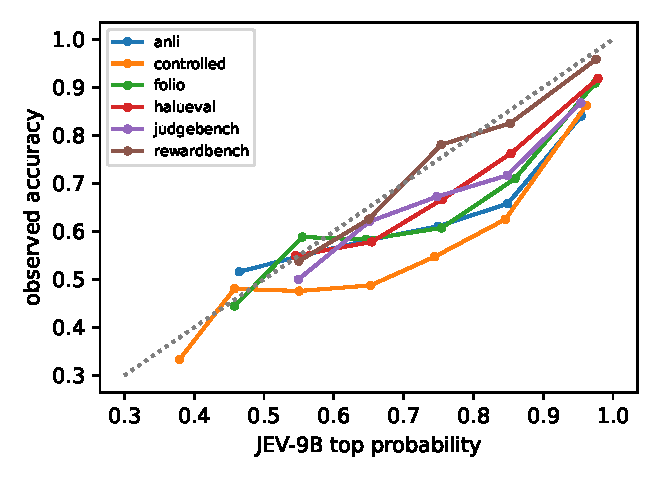
\includegraphics[width=0.55\linewidth]{figures/calibration.pdf}
\caption{Reliability of JEV-9B System~1's top probability by task family (bins with at least 15 items).}
\label{fig:calibration}
\end{figure}
A decision model's selling point is its probability, so we test it out of distribution (Table~\ref{tab:calibration}, Figure~\ref{fig:calibration}).
On RewardBench the top probability is well calibrated (mean confidence 88.5\% against 87.0\% accuracy; ECE 0.026).
On the reasoning panels it is systematically overconfident by 6.8 (FOLIO) to 10.7 (controlled) points, with ECE around 0.10---two orders of magnitude above the 0.0007 the model card reports on its in-distribution test set.
Confidence remains informative for ranking (it is what makes the JEV-H gate work), but a deployment should not read a 0.8 from JEV-9B on a reasoning task as an 80\% chance of being right without recalibrating on its own data.

\paragraph{Threshold sensitivity (exploratory).}
\begin{figure}[t]
\centering
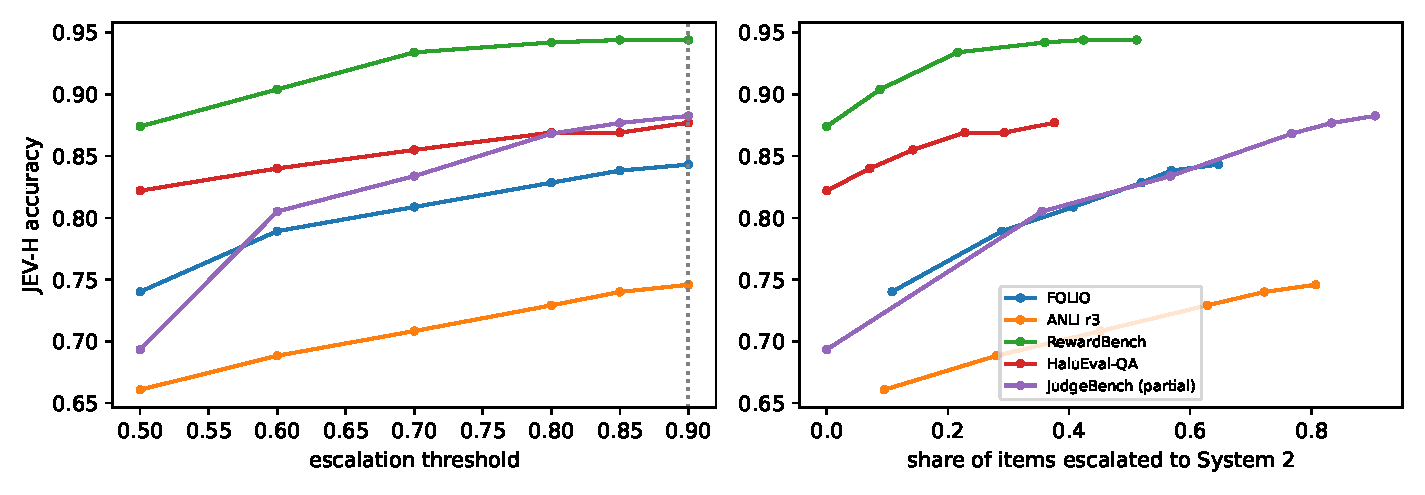
\includegraphics[width=\linewidth]{figures/threshold.pdf}
\caption{JEV-H as the escalation threshold varies (exploratory; the preregistered threshold is 0.90, dotted). Left: accuracy against threshold. Right: accuracy against the share of items escalated to System~2.}
\label{fig:threshold}
\end{figure}
The preregistered threshold of 0.90 was fixed a priori; Figure~\ref{fig:threshold} shows what lower thresholds would have bought, using the System~2 answers already collected.
Most of the gain arrives early: on RewardBench a threshold of 0.70 reaches 93.4\% while escalating 22\% of items (0.90: 94.4\% at 51\%), and on JudgeBench 0.60 already lifts accuracy from 69.3\% to 80.5\% at 36\% escalation.
On FOLIO and ANLI the curve keeps rising to 0.90, because the one-pass model is unsure on most items.
A deployment should choose its threshold from this curve on its own labelled data; \texttt{jevstudy judge} reports it.

\subsection{Robustness}
\label{sec:robust}
\begin{table}[t]
\centering\small
\caption{Option-order reversal (all systems see the reversed list). Flip rate: share of items whose answer, mapped back to the original order, differs from the original answer (\%).}
\label{tab:reversal}
\begin{tabular}{@{}llrrrr@{}}
\toprule
Panel & System & $n$ & Acc.\ orig. & Acc.\ rev. & Flip rate \\
\midrule
FOLIO & JEV-9B S1 & 204 & 69.6 & 68.1 & 5.9 \\
\addlinespace
Controlled base & JEV-9B S1 & 288 & 55.9 & 55.6 & 3.5 \\
\bottomrule
\end{tabular}
\end{table}

Reversing the option list changes System~1's answer on \FlipFolioSone\% of FOLIO items and \FlipCtlSone\% of controlled items (Table~\ref{tab:reversal}), well below the 11.5\% the model card reports for sixteen-option lists; on these three-option tasks position bias is not the main error source.
The frontier arms of this ablation and the max-effort ablation were dropped to limit spending (A5).

\begin{figure}[t]
\centering
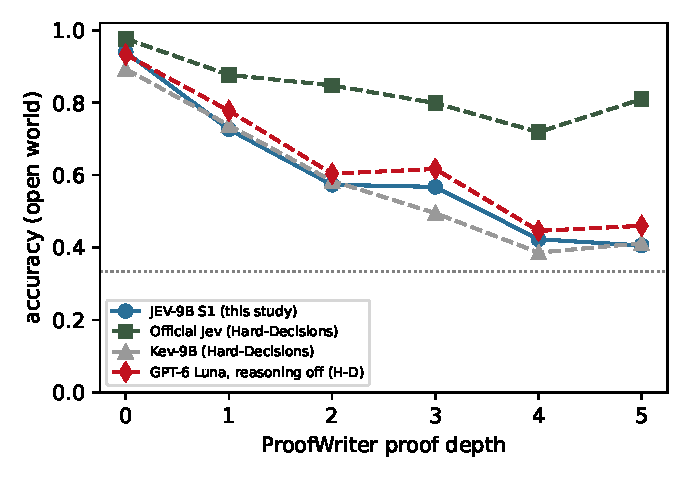
\includegraphics[width=0.62\linewidth]{figures/bridge.pdf}
\caption{ProofWriter open-world accuracy by proof depth: JEV-9B~S1 (this study, 900 items) against official Jev, Kev-9B and GPT-6 Luna without reasoning as published by Hard-Decisions on a different sample of the same strata.}
\label{fig:bridge}
\end{figure}

\begin{table}[t]
\centering\small
\caption{Paired controls at $d{=}3$, $c{=}8$ (48 seeds, \%). Changing: one verified edit flips the gold label. Preserving: renamed entities and reordered premises, same label. ``Changed'' = answer differs from the base answer; ``Both'' = correct on base and edited item; ``Invariant'' = same answer as base.}
\label{tab:controls}
\begin{tabular}{@{}lrrrrrr@{}}
\toprule
& Base & \multicolumn{3}{c}{Decision-changing} & \multicolumn{2}{c}{Decision-preserving} \\
System & acc. & acc. & changed & both & acc. & invariant \\
\midrule
JEV-9B S1 & 40 & 58 & 48 & 23 & 31 & 58 \\
JEV-9B S2 & 100 & 100 & 100 & 100 & 100 & 100 \\
JEV-H harness & 98 & 98 & 98 & 96 & 98 & 96 \\
Astra (high) & 100 & 100 & 100 & 100 & 100 & 100 \\
Fable (high) & 100 & 100 & 100 & 100 & 100 & 100 \\
\bottomrule
\end{tabular}
\end{table}

\begin{table*}[t]
\centering\small
\caption{Selection rules (H3). Leave-one-family-out over five families: mean held-out accuracy (\%), number of folds within 2 points of always-frontier, share of items sent to JEV-9B (\%), and total cost relative to always-frontier. Unseen template: rules fit on everything except controlled template T2, evaluated on T2 items.}
\label{tab:routing}
\begin{tabular}{@{}llrrrrrr@{}}
\toprule
& & \multicolumn{4}{c}{Leave one family out} & \multicolumn{2}{c}{Unseen template T2} \\
Frontier & Policy & Acc. & Within 2 pt & To JEV & Cost ratio & Acc. & To JEV \\
\midrule
Astra & Always JEV-9B & 71.5 & 0/6 & 100 & 0.01 & 49.3 & 100 \\
 & Always frontier & 90.1 & 6/6 & 0 & 1.00 & 100.0 & 0 \\
 & Length only & 90.1 & 6/6 & 1 & 1.00 & 100.0 & 0 \\
 & Family lookup & 90.1 & 6/6 & 0 & 1.00 & 100.0 & 0 \\
 & JEV-9B confidence gate & 87.6 & 4/6 & 45 & 0.67 & 95.1 & 26 \\
 & Feature rule & 87.7 & 4/6 & 19 & 0.84 & 100.0 & 0 \\
 & Feature rule + conf. & 89.3 & 4/6 & 17 & 0.88 & 100.0 & 0 \\
 & Oracle (unattainable) & 93.4 & 6/6 & 78 & 0.25 & 100.0 & 49 \\
\midrule
Fable & Always JEV-9B & 71.5 & 1/6 & 100 & 0.01 & 49.3 & 100 \\
 & Always frontier & 90.9 & 6/6 & 0 & 1.00 & 100.0 & 0 \\
 & Length only & 90.9 & 6/6 & 0 & 1.00 & 100.0 & 0 \\
 & Family lookup & 90.9 & 6/6 & 0 & 1.00 & 100.0 & 0 \\
 & JEV-9B confidence gate & 88.5 & 1/6 & 45 & 0.66 & 95.1 & 26 \\
 & Feature rule & 87.0 & 4/6 & 23 & 0.74 & 100.0 & 0 \\
 & Feature rule + conf. & 88.6 & 4/6 & 21 & 0.78 & 100.0 & 0 \\
 & Oracle (unattainable) & 94.3 & 6/6 & 77 & 0.27 & 100.0 & 49 \\
\bottomrule
\end{tabular}
\end{table*}

\begin{table}[t]
\centering\small
\caption{ProofWriter bridge (A2, exploratory). JEV-9B~S1 accuracy (\%) on 900 open-world items (50 per depth $\times$ label) with Hard-Decisions' task wording, beside official Jev, Kev-9B and GPT-6 Luna (reasoning off) as published by Hard-Decisions on a different sample of the same strata. JEV-9B by label: true 54.2, false 57.3, unknown 71.1.}
\label{tab:bridge}
\begin{tabular}{@{}rrrcrrr@{}}
\toprule
Depth & $n$ & JEV-9B S1 & 95\% CI & Official Jev & Kev-9B & Luna (off) \\
\midrule
0 & 150 & 94.0 & [89.0, 96.8] & 97.7 & 89.3 & 93.3 \\
1 & 150 & 72.7 & [65.0, 79.2] & 87.7 & 73.8 & 77.8 \\
2 & 150 & 57.3 & [49.3, 65.0] & 84.8 & 58.4 & 60.4 \\
3 & 148 & 56.8 & [48.7, 64.5] & 79.9 & 49.5 & 61.7 \\
4 & 149 & 42.3 & [34.6, 50.3] & 71.9 & 38.6 & 44.6 \\
5 & 143 & 40.6 & [32.9, 48.8] & 81.0 & 41.2 & 46.0 \\
\bottomrule
\end{tabular}
\end{table}

\begin{table}[t]
\centering\small
\caption{Accuracy (\%) on inputs of at most / more than 1{,}024 JEV-9B tokens, the length on which JEV-9B was trained. Only panels with long inputs are shown.}
\label{tab:length}
\begin{tabular}{@{}lcccccc@{}}
\toprule
Panel & $n$ short/long & JEV-9B S1 & JEV-9B S2 & JEV-H & Astra & Fable \\
\midrule
JudgeBench (partial) & 54 / 292 & 64.8 / 68.8 & 73.5 / 87.9 & 87.0 / 88.4 & 88.9 / 95.5 & 94.4 / 94.2 \\
RewardBench & 2778 / 206 & 87.2 / 85.0 & 92.4 / 89.5 & 94.3 / 96.4 & 93.9 / 92.9 & 89.8 / 96.4 \\
\bottomrule
\end{tabular}
\end{table}

\subsection{Discussion details}
\paragraph{Why depth did not matter.}
We expected the one-pass model to degrade with each additional dependent step, as models without reasoning do on ProofWriter~\citep{harddecisions2026}.
On our fragment, it was already far from ceiling at depth one, and its errors were dominated by a reluctance to answer \emph{Unknown}---a known difficulty~\citep{qmfol2026,harddecisions2026}--- and by instability under renaming and reordering.
One reading is that a one-pass reader of an unfamiliar formal fragment does not follow rule chains at all, so their length is irrelevant; on ProofWriter, whose natural vocabulary it saw in distillation, depth does matter (Appendix Table~\ref{tab:bridge}).
A depth effect may therefore require familiarity with the surface form before it can appear.

\paragraph{Cost, measured.}
At high effort both frontier models reasoned briefly---tens to a few hundred output tokens per item---so the frontier cost per decision was \$0.002--0.04, far below the planning estimates.
The economic case for a decision model is thus not that frontier reasoning is unaffordable, but that it is 25--290 times more expensive per decision, which matters at evaluation volume.
The whole study, including every API call, cost \$\ApiTotal{} in API fees plus a single rented GPU.

\paragraph{When is the frontier worth paying for?}
\paragraph{When is the frontier worth paying for?}
\begin{table}[t]
\centering\small
\caption{Break-even cost of one error. With expected loss $=$ cost per decision $+$ $P(\text{error})\times c$, paying for the frontier instead of the JEV-9B configuration is worth it only when an error costs more than $c^*=\Delta\text{cost}/\Delta\text{accuracy}$. ``never'': the JEV-9B configuration is at least as accurate and cheaper.}
\label{tab:breakeven}
\begin{tabular}{@{}llrr@{}}
\toprule
Panel & Cheap system & $c^*$ vs.\ Astra & $c^*$ vs.\ Fable \\
\midrule
FOLIO & JEV-9B S1 & \$0.052 & \$0.057 \\
 & JEV-H harness & \$0.346 & \$0.190 \\
ANLI r3 & JEV-9B S1 & \$0.065 & \$0.057 \\
 & JEV-H harness & \$1.91 & \$0.251 \\
Controlled & JEV-9B S1 & \$0.013 & \$0.018 \\
 & JEV-H harness & \$0.162 & \$0.233 \\
JudgeBench (partial) & JEV-9B S1 & \$0.083 & \$0.162 \\
 & JEV-H harness & \$0.327 & \$0.677 \\
RewardBench & JEV-9B S1 & \$0.057 & \$0.177 \\
 & JEV-H harness & never & never \\
HaluEval-QA & JEV-9B S1 & \$0.030 & \$0.033 \\
 & JEV-H harness & \$0.070 & \$0.057 \\
\bottomrule
\end{tabular}
\end{table}

Expected loss per decision is its cost plus the probability of an error times what an error costs; paying for the frontier is worth it exactly when an error costs more than $c^*=\Delta\text{cost}/\Delta\text{accuracy}$ (Table~\ref{tab:breakeven}).
Against one-pass JEV-9B, $c^*$ is between one and eighteen cents on every panel: whenever a wrong decision costs a user more than a few cents---a mislabelled support ticket, an accepted bad answer in an evaluation set---the frontier's accuracy pays for itself.
JEV-H raises $c^*$ by 2--30$\times$ (HaluEval to ANLI), and on RewardBench to \emph{never}: there the harness is both more accurate and cheaper than either frontier.
The decision rule is established decision analysis, not a contribution; the measured inputs to it are.

\subsection{Threats to validity}
\label{sec:threats}

\paragraph{Construct: a student, not the teacher.}
Every decision-model result is about JEV-9B, a community distillation of Jev~1.13 that its authors report trails the teacher on gold accuracy at every option count, flips 11.5\% of sixteen-option answers under reordering (teacher: 7.0\%), and has a KL of 0.234 on unseen task families.
The ProofWriter bridge (Section~\ref{sec:bridge}) compares the two only at the level of depth-stratified accuracy on different samples of the same strata; it bounds, but does not measure, how far our conclusions transfer to official Jev.

\paragraph{Construct: the controlled fragment.}
The fragment uses unary predicates, single-premise rules and invented words.
It isolates dependency depth from length and vocabulary by construction, at the cost of naturalness; its conclusions apply to this fragment, and the public panels are where naturalness is tested.
Automated round-trip parsing guarantees that each sentence states its formula, but not that a human would read the templates the same way; we could not run the planned blinded human review.

\paragraph{Internal: matched prompts are not matched interfaces.}
All systems see identical task content, but JEV-9B consumes it through a typed template it was trained on, while the frontier models receive free text with a schema-constrained answer.
A prompt engineered separately for each system could change accuracies; we report the common-prompt comparison only, and one-sided prompt tuning would not be a fair alternative.
System~2 answers in free text that we parse; its parse failures are counted as errors.

\paragraph{Internal: provider-side variation.}
Frontier models run on hidden infrastructure whose routing and versions we cannot control; we logged the resolved model on every response and saw no change, but services may differ between the days of our runs.
Reasoning effort names are not comparable compute across providers.

\paragraph{Statistical.}
FOLIO's 204 rows form only 73 independent stories, so its intervals are wide; no FOLIO-only result can certify a two-point margin.
Repeated hypotheses are Bonferroni-adjusted within declared families; exploratory analyses (A1, A2, G02, length strata) carry no multiplicity control and are labelled as such.
Interval coverage was checked by simulation under a latent-normal model, which may not match real discordance structure.

\paragraph{External: cost and latency.}
JEV-9B's cost is GPU time on one rented A40 at one utilisation level; a different card, batch size or utilisation changes it by integer factors.
Frontier prices are dated list prices; negotiated or cached pricing would lower them.
JEV-9B latency excludes a network hop; frontier latency includes one.

\FloatBarrier
\section{Preregistration, Amendments and Deviations}
\label{app:prereg}
The full preregistration is \texttt{research/PREREGISTRATION.md} in the repository.
It was committed publicly (commit \texttt{9908524}) after the 24-item development pilot and the 48-item controlled development panel, and before any final-panel call.
Amendments A1 (deep controlled extension) and A2 (ProofWriter bridge) were committed (\texttt{88a8eff}) while final runs were in progress and before any final-panel outcome was analysed; both are exploratory.
Deviations from the original plan, all declared before final calls:
(1) official Jev was replaced by the community distillation JEV-9B because no official access existed;
(2) Banking77 was presented with sixteen candidates and made secondary, then dropped under A5;
(3) JudgeBench was made secondary because its inputs exceed JEV-9B's training length;
(4) the evidence-sufficiency factor (G02) was made exploratory;
(5) blinded human review of controlled items was replaced by automated round-trip parsing and two independent reference scorers;
(6) accuracy runs used synchronous calls, with batch prices reported as a derived view;
(7) the same-weights System~2 arm was added.

\paragraph{Operational incident.}
During the pilot a code-synchronisation command deleted the raw result files and the spend ledger on the pod.
Every completed, non-error response had been cached with its usage and cost, so the results and ledger were rebuilt from the cache (\texttt{jevstudy restore}); panels were regenerated, and all seven panel task-hash digests matched the originals exactly.
No paid call was repeated; the only response not recoverable was a \$0 credit-balance error from the first Fable call.
The development-ID seal is the committed seed and code (\texttt{248d223}), which predates every model call.

\section{Prompts and Request Wrappers}
\label{app:prompts}
\paragraph{Canonical text (frontier models).} For controlled item \texttt{ctl-424242-d1-c0} (gold: True, depth 1):
\begin{quote}\footnotesize\ttfamily
Task: Decide whether the statement follows from the facts and rules, using only the facts and rules. Choose True if they entail the statement, False if they entail its negation, and Unknown if neither follows.\\[3pt]
Evidence:\\
Facts and rules:\\
1. If someone is not ulvarn, then they are not zelvic.\\
2. If someone is not sombic, then they are narlin.\\
3. If someone is not delmor, then they are not tembic.\\
4. If someone is gostal, then they are not brelic.\\
5. If someone is gremal, then they are fenric.\\
6. If someone is not brelic, then they are not rustal.\\
7. Perry is mavric.\\
8. Perry is not vexlan.\\
9. If someone is not vexlan, then they are tembic.\\
10. If someone is not nostel, then they are welbic.\\[3pt]
Question: Statement: Perry is tembic. Is the statement True, False, or Unknown?\\[3pt]
Choices:\\
A) True\\
B) False\\
C) Unknown\\[3pt]
Select the correct choice using the supplied information and task definition. Return the final choice identifier.
\end{quote}
Rule 3 is the distractor chain that ends at the target predicate with the opposite sign; it does not fire because Perry's \textit{delmor} status is never established.

\paragraph{JEV-9B System~1.} The same instructions and evidence form the \texttt{[state]}; the request is a single-token completion constrained to the option verbalisers:
\begin{quote}\footnotesize\ttfamily
{[}kind{]} choice\\
{[}state{]} Task: Decide whether \ldots{} (identical instructions and evidence)\\
{[}question{]} Statement: Perry is tembic. Is the statement True, False, or Unknown?\\
{[}options{]}\\
A) True\\ B) False\\ C) Unknown\\
{[}decision{]}:
\end{quote}

\paragraph{Wrappers.}
OpenAI: \texttt{responses.create(model="gpt-6-astra", input=<canonical text>, reasoning=\{"effort":"high"\}, max\_output\_tokens=32000, text=\{"format":\{"type":"json\_schema","strict":true,"schema":\{answer: enum[A..]\}\}\}, store=false)}.
Anthropic: \texttt{messages.create(model="claude-fable-5-1", max\_tokens=32000, messages=[\{"role":"user","content":<canonical text>\}], output\_config=\{"effort":"high","format":\{"type":"json\_schema","schema":\{answer: enum[A..]\}\}\})}.
JEV-9B System~2: \texttt{chat.completions} on the base model with \texttt{enable\_thinking=true}, the canonical text plus the line \texttt{Respond with JSON \{"answer": "<choice identifier>"\}.}

\section{Controlled Generator Details}
\label{app:generator}
\paragraph{Vocabulary.} Forty invented six-letter predicates (\textit{dravic, florin, gremal, \ldots}) and twenty five-letter names.
\paragraph{Templates.} T1: ``\{E\} is (not) \{a\}.'' / ``If someone is (not) \{b\}, then they are (not) \{h\}.'' T2 (unseen, half of held-out seeds): ``It is known that \{E\} is (not) \{a\}.'' / ``Everyone who is (not) \{b\} is also (not) \{h\}.''
\paragraph{Examples.} The same seed at depth 5 (gold True) chains \textit{not vexlan} $\to$ \textit{delmor} $\to$ \textit{ulvarn} $\to$ \textit{not zelvic} $\to$ \textit{not gremal} $\to$ \textit{tembic} through rules 7, 2, 6, 4 and 3, while rule 5 (\textit{fenric} $\to$ \textit{not tembic}) is the opposite-sign distractor; the evidence has ten numbered lines, as at depth 1.
The decision-changing control for this seed flips the sign of the final chain rule, so the gold label becomes False.
\paragraph{Validation.} For all 416 held-out items and 72 deep-extension items, the brute-force classical scorer and forward chaining agree, measured derivation depth equals designed depth, every grounding is consistent, and every sentence parses back to its formula.

\section{Error Examples}
\label{app:examples}
Controlled items that JEV-9B System~1 answers incorrectly and that GPT-6 Astra, Claude Fable~5.1 and JEV-9B System~2 all answer correctly (one per gold label, chosen with a fixed seed).
\paragraph{ctl-424289-d3-c0 (depth 3, 0 irrelevant facts).} Gold: \textbf{Unknown}; JEV-9B~S1: \textbf{True} (confidence 80.2\%); Astra, Fable and System~2: correct.
\begin{quote}\footnotesize 1. It is known that Finch is not welbic. \\ 2. Everyone who is not hobrin is also gremal. \\ 3. Everyone who is sombic is also not narlin. \\ 4. It is known that Finch is kombar. \\ 5. Everyone who is not wumpic is also sombic. \\ 6. Everyone who is not florin is also not gremal. \\ 7. Everyone who is not vexlan is also not florin. \\ 8. Everyone who is welbic is also bontic. \\ 9. Everyone who is not kelpid is also not delmor. \\ 10. Everyone who is bontic is also not hobrin. \\[2pt] Statement: Finch is gremal. Is the statement True, False, or Unknown?\end{quote}
\paragraph{ctl-424266-d5-c8 (depth 5, 8 irrelevant facts).} Gold: \textbf{True}; JEV-9B~S1: \textbf{False} (confidence 39.6\%); Astra, Fable and System~2: correct.
\begin{quote}\footnotesize 1. If someone is not tarvin, then they are kelpid. \\ 2. Mason is not vexlan. \\ 3. Avery is lumbic. \\ 4. If someone is not welbic, then they are not tarvin. \\ 5. If someone is not lintor, then they are not welbic. \\ 6. Hayes is kelpid. \\ 7. Wynne is not yorbin. \\ 8. Tatum is not vintor. \\ 9. If someone is not yorbin, then they are not vintor. \\ 10. If someone is not yelmar, then they are not lumbic. \\ 11. Blake is not delmor. \\ 12. Devon is not tarvin. \\ 13. Blake is zelvic. \\ 14. Reese is vexlan. \\ 15. Quinn is lumbic. \\ 16. If someone is not morvex, then they are vexlan. \\ 17. If someone is zelvic, then they are not lintor. \\ 18. If someone is kelpid, then they are lumbic. \\[2pt] Statement: Blake is lumbic. Is the statement True, False, or Unknown?\end{quote}
\paragraph{ctl-424279-d1-c8 (depth 1, 8 irrelevant facts).} Gold: \textbf{False}; JEV-9B~S1: \textbf{True} (confidence 63.1\%); Astra, Fable and System~2: correct.
\begin{quote}\footnotesize 1. It is known that Jesse is not gostal. \\ 2. Everyone who is cravel is also zorvin. \\ 3. It is known that Sasha is rustal. \\ 4. Everyone who is pexton is also not delmor. \\ 5. Everyone who is not tarvin is also gostal. \\ 6. It is known that Casey is fenric. \\ 7. It is known that Reese is not morvex. \\ 8. It is known that Logan is pexton. \\ 9. It is known that Hayes is not gostal. \\ 10. Everyone who is fenric is also not lintor. \\ 11. It is known that Noble is not morvex. \\ 12. Everyone who is not ribrel is also not morvex. \\ 13. It is known that Ellis is not ribrel. \\ 14. It is known that Ellis is xantic. \\ 15. Everyone who is not lintor is also rustal. \\ 16. Everyone who is zorvin is also morvex. \\ 17. It is known that Tatum is delmor. \\ 18. Everyone who is not delmor is also not ulvarn. \\[2pt] Statement: Ellis is morvex. Is the statement True, False, or Unknown?\end{quote}


\section{Reproducibility}
\label{app:repro}
Everything needed to reproduce the study is in the public repository: the package (\texttt{src/jevstudy}), tests (22 tests covering gold exclusion, prompt parity, cache keys, cost accounting, retries, scorer agreement and interval behaviour), pinned panel builders, manifests (dataset sources with SHA-256, model revisions, rate card, development IDs, latency subset), the preregistration, and RunPod scripts.
\begin{quote}\footnotesize\ttfamily
runpod/pod.sh create \&\& runpod/pod.sh sync \&\& runpod/pod.sh secrets\\
runpod/pod.sh ssh 'bash /workspace/jev/runpod/setup\_remote.sh \&\& bash /workspace/jev/runpod/start\_vllm.sh'\\
jevstudy prepare; jevstudy variants; jevstudy amendments\\
bash runpod/full\_run.sh\\
python -m jevstudy.paper\_assets --root . --out research-paper
\end{quote}
Raw dataset text is not redistributed; the builders download it from pinned sources.
Item-level predictions (task IDs, answers, correctness, usage and cost) are released in \texttt{results/final\_item\_level.csv}.


\section{Additional Tables}
\label{app:tables}
\begin{table*}[t]
\centering\small
\caption{Accuracy and cost on every panel. Accuracy in \%, 95\% Wilson interval; failures are scored incorrect.
Cost: USD per 1{,}000 decisions at list price (frontiers: billed tokens; JEV-9B S1: sequential GPU seconds; S2: all pod time spanning System-2 runs divided by System-2 items, a conservative upper estimate; JEV-H: two S1 calls plus S2 on escalated items).
Output tokens include reasoning. Controlled = 288 base items (48 seeds $\times$ 6 conditions).}
\label{tab:main}
\begin{tabular}{@{}llrrcrrr@{}}
\toprule
Panel & System & $n$ & Acc. & 95\% CI & Fail & \$/1k & Out tok. \\
\midrule
FOLIO & JEV-9B S1 & 204 & 69.6 & [63.0, 75.5] & 0 & 0.041 & 0 \\
 & JEV-9B S2 & 204 & 85.8 & [80.3, 89.9] & 0 & 0.609 & 3982 \\
 & JEV-H harness & 204 & 84.3 & [78.7, 88.7] & 0 & 0.483 & 0 \\
 & Astra (high) & 204 & 86.8 & [81.4, 90.7] & 0 & 8.97 & 135 \\
 & Fable (high) & 204 & 90.2 & [85.3, 93.6] & 0 & 11.68 & 131 \\
\addlinespace
ANLI r3 & JEV-9B S1 & 1200 & 64.2 & [61.5, 66.9] & 0 & 0.045 & 0 \\
 & JEV-H harness & 1200 & 74.6 & [72.0, 77.0] & 0 & 0.623 & 0 \\
 & Astra (high) & 1200 & 74.9 & [72.4, 77.3] & 0 & 7.00 & 98 \\
 & Fable (high) & 1200 & 77.3 & [74.9, 79.6] & 0 & 7.52 & 49 \\
\addlinespace
Controlled & JEV-9B S1 & 288 & 55.9 & [50.1, 61.5] & 0 & 0.037 & 0 \\
 & JEV-9B S2 & 288 & 100.0 & [98.7, 100.0] & 0 & 0.609 & 2239 \\
 & JEV-H harness & 288 & 96.9 & [94.2, 98.3] & 0 & 0.572 & 0 \\
 & Astra (high) & 288 & 100.0 & [98.7, 100.0] & 0 & 5.65 & 51 \\
 & Fable (high) & 288 & 100.0 & [98.7, 100.0] & 0 & 7.87 & 33 \\
\addlinespace
JudgeBench (partial) & JEV-9B S1 & 346 & 68.2 & [63.1, 72.9] & 0 & 0.153 & 0 \\
 & JEV-H harness & 346 & 88.2 & [84.3, 91.1] & 0 & 1.19 & 0 \\
 & Astra (high) & 346 & 94.5 & [91.6, 96.5] & 0 & 22.01 & 137 \\
 & Fable (high) & 346 & 94.2 & [91.2, 96.2] & 1 & 42.28 & 362 \\
\addlinespace
RewardBench & JEV-9B S1 & 2984 & 87.0 & [85.8, 88.2] & 0 & 0.170 & 0 \\
 & JEV-H harness & 500 & 94.4 & [92.0, 96.1] & 0 & 0.654 & 0 \\
 & Astra (high) & 500 & 93.8 & [91.3, 95.6] & 0 & 4.01 & 60 \\
 & Fable (high) & 500 & 90.2 & [87.3, 92.5] & 25 & 5.78 & 46 \\
\addlinespace
HaluEval-QA & JEV-9B S1 & 1000 & 82.7 & [80.2, 84.9] & 0 & 0.096 & 0 \\
 & JEV-H harness & 1000 & 87.7 & [85.5, 89.6] & 0 & 0.424 & 0 \\
 & Astra (high) & 1000 & 90.6 & [88.6, 92.3] & 0 & 2.45 & 48 \\
 & Fable (high) & 1000 & 93.3 & [91.6, 94.7] & 0 & 3.64 & 31 \\
\bottomrule
\end{tabular}
\end{table*}

\begin{table}[t]
\centering\small
\caption{Evaluated systems. Official TypeSafe Jev was not evaluated: no API access was available and its weights are not public. Every claim refers to JEV-9B, a community distillation of Jev~1.13.}
\label{tab:systems}
\begin{tabularx}{\linewidth}{@{}llX@{}}
\toprule
Key & Model (revision) & Configuration \\
\midrule
\texttt{jev9b-s1} & autotrust/JEV-9B (\texttt{b63f651}) & System~1 choice head via vLLM~0.31.0 LoRA; bias + temperature 0.984 client-side; no truncation (context 32{,}768) \\
\texttt{jev9b-s2} & same weights, base \texttt{lm\_head} & Qwen3.5-9B, \texttt{enable\_thinking}, $T{=}0.6$, top-$p{=}0.95$, 16k tokens; free-text answer parsed \\
\texttt{astra-high} & \texttt{gpt-6-astra} & Responses API, \texttt{reasoning.effort=high}, 32k output, strict JSON schema, no tools \\
\texttt{fable-high} & \texttt{claude-fable-5-1} & Messages API, adaptive thinking (always on), \texttt{effort=high}, 32k output, JSON schema, no tools, no fallback \\
\bottomrule
\end{tabularx}
\end{table}


\begin{table*}[t]
\centering\small
\caption{Leave-one-family-out detail: held-out accuracy (\%) / share routed to JEV-9B (\%) per policy.}
\label{tab:routingdetail}
\begin{tabular}{@{}llcccccc@{}}
\toprule
Frontier & Held-out family & Always JEV & Always frontier & Conf.\ gate & Feature rule & Rule + conf. & Oracle \\
\midrule
Astra & anli & 64.2/100 & 74.9/0 & 73.7/27 & 74.9/0 & 74.7/4 & 82.9/81 \\
Astra & controlled & 55.9/100 & 100.0/0 & 95.1/28 & 100.0/0 & 100.0/0 & 100.0/56 \\
Astra & folio & 69.6/100 & 86.8/0 & 84.8/42 & 86.8/0 & 87.7/7 & 90.7/79 \\
Astra & halueval & 82.7/100 & 90.6/0 & 89.2/70 & 82.8/97 & 88.1/81 & 91.6/91 \\
Astra & judgebench & 68.2/100 & 94.6/0 & 88.8/34 & 88.0/19 & 91.7/10 & 97.7/70 \\
Astra & rewardbench & 88.4/100 & 93.8/0 & 94.0/68 & 93.8/0 & 93.8/0 & 97.2/91 \\
Fable & anli & 64.2/100 & 77.3/0 & 74.8/31 & 77.3/0 & 77.2/4 & 85.2/79 \\
Fable & controlled & 55.9/100 & 100.0/0 & 95.1/28 & 100.0/0 & 100.0/0 & 100.0/56 \\
Fable & folio & 69.6/100 & 90.2/0 & 87.3/42 & 90.2/0 & 90.2/12 & 91.7/78 \\
Fable & halueval & 82.7/100 & 93.3/0 & 90.9/72 & 82.9/99 & 89.7/80 & 93.8/89 \\
Fable & judgebench & 68.2/100 & 94.3/0 & 88.5/34 & 81.4/39 & 84.5/32 & 97.4/71 \\
Fable & rewardbench & 88.4/100 & 90.2/0 & 94.2/64 & 90.2/0 & 90.2/0 & 97.6/91 \\
\bottomrule
\end{tabular}
\end{table*}

\begin{table}[t]
\centering\small
\caption{Study cost ledger. API rows: billed usage at list price on the final, ablation and exploratory panels (development calls appear only in the ledger total). Ledger total for all API calls including probes: \$65.04. System~2 pod-hours over its run windows: 2.0 h (\$1.16 at \$0.59/h); the whole pod's rental is reported in the text.}
\label{tab:ledger}
\begin{tabular}{@{}llrrrr@{}}
\toprule
System & Family & Calls & In (M tok) & Out (M tok) & USD \\
\midrule
Astra (high) & anli & 1200 & 0.25 & 0.118 & 8.40 \\
Astra (high) & controlled & 488 & 0.16 & 0.025 & 2.88 \\
Astra (high) & folio & 204 & 0.05 & 0.028 & 1.83 \\
Astra (high) & halueval & 1000 & 0.25 & 0.048 & 2.45 \\
Astra (high) & judgebench & 349 & 0.53 & 0.048 & 7.65 \\
Astra (high) & rewardbench & 500 & 0.25 & 0.030 & 2.00 \\
Fable (high) & anli & 1200 & 0.61 & 0.059 & 9.02 \\
Fable (high) & controlled & 488 & 0.32 & 0.017 & 4.01 \\
Fable (high) & folio & 204 & 0.11 & 0.027 & 2.38 \\
Fable (high) & halueval & 1000 & 0.57 & 0.031 & 3.64 \\
Fable (high) & judgebench & 349 & 0.84 & 0.126 & 14.68 \\
Fable (high) & rewardbench & 500 & 0.46 & 0.023 & 2.89 \\
\bottomrule
\end{tabular}
\end{table}


\section*{NeurIPS Paper Checklist}
\addcontentsline{toc}{section}{NeurIPS Paper Checklist}
\small

\begin{enumerate}[leftmargin=1.4em,itemsep=3pt]
\item \textbf{Claims.} Do the main claims in the abstract and introduction accurately reflect the paper's contributions and scope?
\textbf{Yes.} Every claim names JEV-9B (not official Jev), the two frontier configurations and the panels on which it was measured; the failed depth hypothesis and the student--teacher gap are stated in the abstract (Sections~\ref{sec:controlled-results},~\ref{sec:bridge}).

\item \textbf{Limitations.} \textbf{Yes.} Section~\ref{sec:threats} (threats to validity) and the Limitations subsection.

\item \textbf{Theory, assumptions and proofs.} \textbf{NA.} The paper makes no theoretical claims; the decision rule is established decision analysis.

\item \textbf{Experimental result reproducibility.} \textbf{Yes.} Exact model revisions, API parameters, prompts and wrappers (Appendix~\ref{app:prompts}), dataset commits and SHA-256 hashes, seeds, and the full pipeline (Appendix~\ref{app:repro}).

\item \textbf{Open access to data and code.} \textbf{Yes.} Code, preregistration, controlled panels, item-level predictions and manifests are public; licensed benchmark text is rebuilt from pinned sources rather than redistributed.

\item \textbf{Experimental setting and details.} \textbf{Yes.} Sections~\ref{sec:design}--\ref{sec:protocol}; no model was trained or tuned, and the only free parameter of the harness (threshold 0.90) was fixed a priori.

\item \textbf{Experiment statistical significance.} \textbf{Yes.} Paired Newcombe score intervals or seed/question-clustered bootstrap intervals, Bonferroni-adjusted within preregistered families, with simulated coverage reported (Section~\ref{sec:stats}).

\item \textbf{Experiments compute resources.} \textbf{Yes.} One NVIDIA A40 (48\,GB) rented on RunPod at \$0.59/h for all serving, clients and analysis; API spend \$\ApiTotal{} in total; per-panel costs in Table~\ref{tab:main} and Appendix Table~\ref{tab:ledger}.

\item \textbf{Code of ethics.} \textbf{Yes.} The research uses public benchmarks and public models; no human subjects or personal data.

\item \textbf{Broader impacts.} \textbf{Yes.} Cheaper automated evaluation can widen access to careful model testing; it can also encourage over-reliance on a judge that, as shown here, fails on reasoning-heavy correctness judgements. We therefore release the tool with confidence-gated escalation and a protocol for validating it on the user's own labelled data, and state where it should not be used.

\item \textbf{Safeguards.} \textbf{NA.} No high-risk model or dataset is released; the judging API wraps an existing open model.

\item \textbf{Licences for existing assets.} \textbf{Yes.} JEV-9B (Apache-2.0), FOLIO (CC-BY-SA-4.0), ANLI (CC-BY-NC-4.0), JudgeBench (MIT), RewardBench (ODC-BY), HaluEval (Apache-2.0), ProofWriter (CC-BY-4.0), Banking77 (CC-BY-4.0); all cited, none redistributed.

\item \textbf{New assets.} \textbf{Yes.} The controlled dependency panel, generator and reference scorers, the JEV-H harness and the judging API are documented in the repository under Apache-2.0.

\item \textbf{Crowdsourcing and human subjects.} \textbf{NA.}

\item \textbf{IRB approvals.} \textbf{NA.}

\item \textbf{Declaration of LLM usage.} \textbf{Yes.} The study evaluates LLMs as its subject. An AI coding assistant was used to implement the software and draft the manuscript under the author's direction; all design decisions, preregistration and reported numbers are traceable to the committed code and data.
\end{enumerate}


\end{document}
